% Template adapted from https://github.com/sylvainschmitt/PhD/tree/master/documents/thesis/latex/template.latex

%%% STYLE %%%
\documentclass[12pt,twoside,a4paper, a]{article}



%%% PACKAGES %%%

% fonts
\usepackage{lmodern}
% \usepackage{anyfontsize}

% pdf
\usepackage{pdfpages}

% formulae
\usepackage{amssymb,amsmath}
\usepackage{ifxetex,ifluatex}
\usepackage{fixltx2e}
\usepackage[T1]{fontenc}
\usepackage[utf8]{inputenc}

% Tables
% pacakges for kableextra
\usepackage{booktabs}
\usepackage{longtable}
\usepackage{array}
\usepackage{multirow}
\usepackage{wrapfig}
\usepackage{float}
\usepackage{colortbl}
\usepackage{pdflscape}
\usepackage{tabu}
\usepackage{threeparttable}
\usepackage{threeparttablex}
\usepackage[normalem]{ulem}
\usepackage{makecell}
\usepackage{xcolor}
% \usepackage{longtable,booktabs}
% Fix footnotes in tables (requires footnote package)
\IfFileExists{footnote.sty}{\usepackage{footnote}\makesavenoteenv{long table}}{}

% graphics

% indent
\IfFileExists{parskip.sty}{%
\usepackage{parskip}
}{% else
\setlength{\parindent}{0pt}
\setlength{\parskip}{6pt plus 2pt minus 1pt}
}

% prevent overfull lines
\setlength{\emergencystretch}{3em}  
\providecommand{\tightlist}{%
\setlength{\itemsep}{0pt}\setlength{\parskip}{0pt}}

\setcounter{secnumdepth}{0}

% set default figure placement to htbp
\makeatletter 
\def\fps@figure{htbp}
\makeatother

% set default table placement to htbp
\makeatletter 
\def\fps@table{htbp}
\makeatother

% code highlights

% background image added by V.V.
\usepackage{eso-pic}
\newcommand\BackgroundIm{
\put(0,0){
  \parbox[b][\paperheight]{\paperwidth}{%
    \vfill
    \centering
    
\includegraphics[height=\paperheight,width=\paperwidth]{img/background.jpg}%
    \vfill
}}}

% packages added by V.V.
\usepackage{lettrine}
\usepackage{caption}

% For Pandoc 2.11+, added by V.V. from thesisdown
\newlength{\cslhangindent}
\setlength{\cslhangindent}{1.5em}
\newenvironment{CSLReferences}[2] % #1 hanging-ident, #2 entry spacing
 {% don't indent paragraphs
  \setlength{\parindent}{0pt}
  % turn on hanging indent if param 1 is 1
  \ifodd #1 \everypar{\setlength{\hangindent}{\cslhangindent}}\ignorespaces\fi
  % set entry spacing
  \ifnum #2 > 0
  \setlength{\parskip}{#2\baselineskip}
  \fi
 }%
 {}
 
% To pass between YAML and LaTeX, added by V.V. from thesisdown
\def\title#1{\def\title{#1}}
\title{FIABILITÉ DES PROJECTIONS DES MODÈLES D'AIRE DE RÉPARTITION DES ARBRES FORESTIERS}
\def\author#1{\def\author{#1}}
\author{Victor VAN DER MEERSCH}
\def\date#1{\def\date{#1}}
\date{01 Janvier 2001}
\def\supervisor#1{\def\supervisor{#1}}
\supervisor{Isabelle CHUINE}
\def\specialty#1{\def\specialty{#1}}
\specialty{Écologie fonctionnelle et Sciences Agronomiques}
\def\department#1{\def\department{#1}}
\department{UMR 5175 -- Centre d'Ecologie Fonctionnelle et Evolutive - CNRS}

% paragraphs
% beware this make the toc bug if hyperref is placed before
\usepackage{titlesec}
\let\oldsection\section
\renewcommand\section{\clearpage\oldsection}
\titleformat{\section}
{\huge\center\scshape}{\thesection}{1em}{}[{\titlerule[0.5pt]}]
\titleformat*{\subsection}{\LARGE\bfseries}
\titleformat*{\subsubsection}{\Large\bfseries}
\titleformat*{\paragraph}{\large\bfseries\itshape}
\titleformat*{\subparagraph}{\normalsize\itshape}

% hyperlinks (cleverref and colors for UM added by V.V.)
\IfFileExists{upquote.sty}{\usepackage{upquote}}{}
\IfFileExists{microtype.sty}{%
\usepackage[]{microtype}
\UseMicrotypeSet[protrusion]{basicmath} % disable protrusion for tt fonts
}{}
\PassOptionsToPackage{hyphens}{url} % url is loaded by hyperref
\usepackage[unicode=true]{hyperref}
  \PassOptionsToPackage{usenames,dvipsnames}{color} % color is loaded by hyperref
\definecolor{um-red}{RGB}{233,78,82}
\definecolor{um-gray}{RGB}{114,146,162}
\hypersetup{
      colorlinks=true,
    linkcolor=um-red,
    citecolor=um-red,
    urlcolor=um-gray,
      breaklinks=true}
\urlstyle{same} % don't use monospace font for urls
\usepackage[capitalise, nameinlink]{cleveref}

% empty all blank pages created by \cleardoublepage, added by V.V.
\usepackage{emptypage}

% geometry
\usepackage[left=2.5cm,right=2.5cm,top=2cm,bottom=2cm]{geometry}
\renewcommand{\baselinestretch}{1.1}

% Bibliography
\usepackage{natbib}
\bibliographystyle{plainnat}

% citations
\usepackage{epigraph}

%%% BODY %%%
\begin{document}

% First pages
  \begin{titlepage}
    \newpage
    
    \AddToShipoutPicture*{\BackgroundIm}

    \let\footnotesize\small
    \let\footnoterule\relax
    \let \footnote \thanks

    \baselineskip = 1.4\baselineskip

    \begin{center}
    \setcounter{page}{1}
    
    \textbf{\textcolor{um-red}{\large{THÈSE POUR OBTENIR LE GRADE DE DOCTEUR} \\
    \large{DE L'UNIVERSITÉ DE MONTPELLIER} \\ }}
    
    \vspace*{\baselineskip} 
    \normalsize{\textbf{En \specialty}} \\
    \vspace*{\medskipamount} 
    \normalsize{\textbf{Ecole doctorale GAIA}} \\
    \vspace*{\medskipamount}
    \normalsize{\textbf{\department}} \\
    \vspace*{2cm}
    
    \textcolor{um-gray}{\Large{\textbf{\title}} \\ }
    \vspace*{1cm}
    
    \normalsize{\textbf{Présentée par \author}} \\
    \normalsize{\textbf{Le \date}} \\
    \vspace*{\baselineskip}
    
    \normalsize{\textbf{Sous la direction d'\supervisor}} \\
    \vspace*{\fill}
    
    \normalsize{Devant le jury composé de} \\
    \begin{table}[h]
      \centering
      \makebox[0.9\columnwidth]{%
        \begin{tabular}{lllr}
          Prénom NOM             & Titre              & Affiliation                    & \emph{Rôle jury} \\
          Prénom NOM             & Titre              & Affiliation                    & \emph{Rôle jury} \\
          Prénom NOM             & Titre              & Affiliation                    & \emph{Rôle jury} \\
          Prénom NOM             & Titre              & Affiliation                    & \emph{Rôle jury} \\
          Prénom NOM             & Titre              & Affiliation                    & \emph{Rôle jury} \\
          Prénom NOM             & Titre              & Affiliation                    & \emph{Rôle jury} \\
          Prénom NOM             & Titre              & Affiliation                    & \emph{Rôle jury} \\
        \end{tabular}
      }
    \end{table}
    \end{center}
    
    \vspace*{\fill}
    
    \begin{center}
    
\includegraphics[width=0.4\columnwidth]{img/logo-um.png}
    \end{center}
    
  \end{titlepage}

  \cleardoublepage
    \null\vfill
    \begin{figure}[h!]
    \centering
      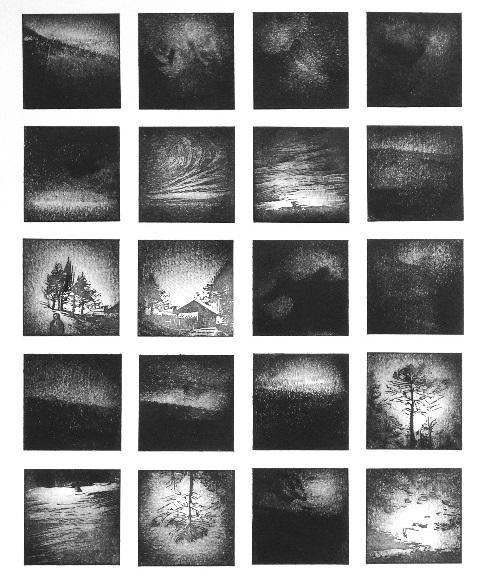
\includegraphics{img/cecile_rescan/cecile_rescan_page.jpg}
      \caption*{Linogravure réalisée par Cécile Rescan}
    \end{figure}
    \vfill\null
  \newpage
  \null\vfill
  {\fontsize{7.5}{8}\selectfont
  \begin{center}
  \textbf{Génomique écologique de l'exploitation de niche et de la performance individuelle chez les arbres forestiers tropicaux} \\
  \end{center} 
  \textbf{Résumé :}
  Les forêts tropicales abritent la plus grande diversité d'espèces au monde, un fait qui reste en partie inexpliqué et dont l'origine est sujette à débat. Même à l'échelle de l'hectare, les forêts tropicales abritent des genres riches en espèces, avec des espèces d’arbres étroitement apparentées qui coexistent en sympatrie. En raison de contraintes phylogénétiques, on s'attend à ce que les espèces étroitement apparentées possèdent des niches et des stratégies fonctionnelles similaires, ce qui questionne les mécanismes de leur coexistence locale. Les espèces étroitement apparentées peuvent former un complexe d'espèces, composé d’espèces morphologiquement similaires ou qui partagent une importante proportion de leur variabilité génétique en raison d'une ascendance commune récente ou d'hybridation, et qui peut résulter d'une radiation écologique adaptative des espèces selon des gradients environnementaux. Malgré le rôle clé des complexes d'espèces dans l'écologie, la diversification et l'évolution des forêts néotropicales, les forces éco-évolutives qui créent et maintiennent la diversité au sein des complexes d'espèces néotropicales restent peu connues. Nous avons exploré la variabilité génétique intraspécifique comme un continuum au sein de populations structurées d'espèces étroitement apparentées, et mesuré son rôle sur la performance individuelle des arbres à travers la croissance dans le temps, tout en tenant compte des effets d'un environnement finement caractérisé au niveau abiotique et biotique. En combinant des inventaires forestiers, des données topographiques, des traits fonctionnels foliaires et des données de capture de gènes dans la station de recherche de Paracou, en Guyane Française, nous avons utilisé la génomique des populations, les analyses d'associations environnementales et génomiques, et la modélisation Bayésienne sur les complexes d'espèces \emph{Symphonia} et \emph{Eschweilera} clade \emph{Parvifolia}. Nous avons montré que les complexes d'espèces d'arbres couvrent l’ensemble des gradients locaux de topographie et de compétition présents dans le site d'étude alors que la plupart des espèces qui les composent présentent une différenciation de niche marquée le long de ces mêmes gradients. Plus précisément, dans les complexes d'espèces étudiés, la diminution de la disponibilité en eau, par exemple depuis les bas-fonds jusqu’aux plateaux, a entraîné une modification des traits fonctionnels foliaires, depuis des stratégies d'acquisition à des stratégies conservatrices, tant entre les espèces qu'au sein de celles-ci. Les espèces de \emph{Symphonia} sont génétiquement adaptées à la distribution de l'eau et des nutriments, elles coexistent donc localement en exploitant un large gradient d'habitats locaux. Inversement, les espèces d'\emph{Eschweilera} sont différentiellement adaptées à la chimie du sol et évitent les habitats les plus humides et hydromorphes. Enfin, les génotypes individuels des espèces de \emph{Symphonia} sont différentiellement adaptés pour se régénérer et croître en réponse à la fine dynamique spatio-temporelle des trouées forestières, avec des stratégies adaptatives de croissance  divergentes le long des niches de succession. Par conséquent, la topographie et la dynamique des trouées forestières entraînent des adaptations spatio-temporelles à fine échelle des individus au sein et entre les espèces des complexes d'espèces \emph{Symphonia} et \emph{Eschweilera} clade \emph{Parvifolia}. Je suggère que les adaptations à la topographie et à la dynamique des trouées forestières favorisent la coexistence des individus au sein et entre les espèces des complexes d'espèces, et peut-être plus généralement entre les espèces d'arbres de forêts matures. Dans l'ensemble, je soutiens le rôle primordial des individus au sein des espèces dans la diversité des forêts tropicales, et suggère que nous devrions élaborer une théorie de l'écologie des communautés en commençant par les individus, car les interactions avec les environnements se produisent après tout au niveau de l’individu. \\

  \textbf{Mots clés :}
  Coexistence des espèces ; Complexe d'espèces ; Distribution des espèces ; Forêts tropicales ; Indice d'encombrement du voisinage ; Indice d'humiditétopographique ; Niche écologique ; Paracou ; Syngameon ; Variabilité intraspécifique \vspace*{\baselineskip}
  \newline\noindent\rule{\textwidth}{0.7pt}

  \begin{center}
  \textbf{Ecological genomics of niche exploitation and individual performance in tropical forest trees} \\
  \end{center} 
  \textbf{Abstract:}
  Tropical forests shelter the highest species diversity worldwide, a fact that remains partly unexplained and the origin of which is subject to debate. Even at the hectare-scale, tropical forests shelter species-rich genera with closely-related tree species coexisting in sympatry. Due to phylogenetic constraints, closely related species are expected to have similar niches and functional strategies, which raises questions on the mechanisms of their local coexistence. Closely related species may form a species complex, defined as morphologically similar species that share large amounts of genetic variation due to recent common ancestry and hybridization, and that can result from ecological adaptive radiation of species segregating along environmental gradients. Despite the key role of species complexes in Neotropical forest ecology, diversification, and evolution, little is known of the eco-evolutionary forces creating and maintaining diversity within Neotropical species complexes. We explored the intraspecific genomic variability as a continuum within structured populations of closely related species, and measured its role on individual tree performance through growth over time, while accounting for effects of a finely-characterized environment at the abiotic and biotic level. Combining tree inventories, LiDAR-derived topographic data, leaf functional traits, and gene capture data in the research station of Paracou, French Guiana, we used population genomics, environmental association analyses, genome-wide association studies and Bayesian modelling on the tree species complexes \emph{Symphonia} and \emph{Eschweilera} clade \emph{Parvifolia}. We showed that the species complexes of Neotropical trees cover all local gradients of topography and competition and are therefore widespread in the study site whereas most of the species within them exhibit pervasive niche differentiation along these same gradients. Specifically, in the species complexes \emph{Symphonia} and \emph{Eschweilera} clade \emph{Parvifolia}, the decrease in water availability due to higher topographic position, e.g., from bottomlands to plateaus, has led to a change in leaf functional traits from acquisitive strategies to conservative strategies, both among and within species. \emph{Symphonia} species are genetically adapted to the distribution of water and nutrients, hence they coexist locally through exploiting a broad gradient of local habitats. Conversely, \emph{Eschweilera} species are differentially adapted to soil chemistry and avoid the wettest, hydromorphic habitats. Last but not least, individual tree genotypes of \emph{Symphonia} species are differentially adapted to regenerate and thrive in response to the fine spatio-temporal dynamics of forest gaps with divergent adaptive growth strategies along successional niches. Consequently, topography and the dynamics of forest gaps drive fine-scale spatio-temporal adaptations of individuals within and among distinct but genetically connected species within the species complexes \emph{Symphonia} and \emph{Eschweilera} clade \emph{Parvifolia}. Fine-scale topography drives genetic divergence and niche differentiation with genetic adaptations among species, while forest gap dynamics maintains genetic diversity with divergent adaptive strategies within species. I suggest that adaptations of tree species and individuals to topography and dynamics of forest gaps promote coexistence within and among species within species complexes, and perhaps among mature forest tree species outside species complexes. Overall, I defend the primordial role of individuals within species in tropical forest diversity, suggesting that we should develop a theory of community ecology starting with individuals, because interactions with environments happen after all at the individual level. 

  \textbf{Keywords:}
  Ecological niche; Intraspecific variability; Neighbourhood crowding index; Paracou; Species coexistence; Species complex; Species distribution; Syngameon; Topographic wetness index;   Tropical forests

  }
  \vfill\null
% 
% \tableofcontents
% \listoftables
% \listoffigures

\newpage

\pagenumbering{arabic}

\hypertarget{remerciements}{%
\section{Remerciements}\label{remerciements}}

\lettrine[lines=8, lraise=0.05, findent=.5em, image=true]{img/cecile_rescan/cecile_rescan_L1.jpg}{} À l'heure où je boucle ces trois années de thèse, je ne peux que me
sentir reconnaissant et chanceux de toutes les personnes qui m'ont
accompagné et dont j'ai croisé la route aussi bien lors de ma thèse que
lors du long du chemin qui m'y a amené. Malgré l'ensemble de la
rédaction que j'ai dû réaliser pour arriver jusque là, il me semble
difficile de remercier exhaustivement les personnes qui ont compté pour
moi, et je m'excuse grandement auprès de celles que j'aurais le malheur
d'oublier. Bien que j'aime à discuter de la biodiversité des arbres
tropicaux, le parcours qui m'a amené jusqu'ici a aussi été l'occasion de
me confronter à une richesse humaine extraordinaire aux quatres coins du
monde !

L'écriture de cette thèse a été un long travail, mais je n'imagine pas
le travail que cela représente de l'évaluer. Je remercie donc les
rapporteurs, \textbf{Xavier Vekemans} et \textbf{Tamara Münkemüller}, ainsi que les
examinateurs, \textbf{Olivier Hardy}, \textbf{Céline Teplitsky}, \textbf{Caroline
Scotti-Saintagne} et \textbf{Marta Benito-Garzón} pour leur intérêt et
l'honneur qu'ils me font de participer à mon jury de thèse.

Je ne pourrais commencer sans citer l'incomparable mais aussi diverse
équipe d'encadrants géniaux qui m'a supervisé et accompagné pendant
trois ans. La richesse de cette thèse commence en effet avec vous qui
venez des quatres coins de l'Europe et du monde. Vous qui vivez chacun
sur votre continent où vous m'avez toujours accueilli au delà de mes
espérances. Vous qui par votre diversité fonctionnelle, autant
académique qu'humaine, créez, à mon humble avis, la richesse et la force
de cet encadrement. Merci à \textbf{Myriam Heuertz} pour ton dynamisme et ta
force pour toujours avancer, que tu as su me prêter dans la réalisation
de mon doctorat. Mais aussi merci pour ce cadre humain que tu as pu
donner à mes trois années: merci pour l'accueil à Bordeaux lors de mon
retour de Guyane, merci pour l'incroyable opportunité que tu m'as donné
avec l'Équateur qui fut involontairement un magnifique cadeau
d'anniversaire, et j'espère pouvoir courir un jour le marathon de
Bordeaux avec toi. Merci à \textbf{Bruno Hérault} d'avoir accepté de partager
ces réflexions incessantes qui m'ont permis d'aller au delà d'où je
pouvais espérer atterrir. Je pense que ta manière de réfléchir et de
toujours remettre en question ce qui peut être trop facilement admis est
primordiale, et j'espère qu'elle restera avec moi au cours de mes futurs
travaux. Merci pour ton humanité qui valorise une existence hors du
travail, merci pour le vélo, les repas, les rigolades et discussions
chez toi, chez moi, au bureau ou sur le terrain. Merci enfin à \textbf{Niklas
Tysklind} d'avoir depuis la première minute et encore aujourd'hui
beaucoup plus cru en moi que moi-même ! À l'heure où nous essayons de
pousser le chapitre 4 vers une revue prestigieuse, je ne peux m'empêcher
de me rappeler que dès le début tu m'a dit le premier, alors que cela me
paraissait totalement inatteignable, que j'arriverais à ce stade. Enfin
en plus du fait que tu es toujours aussi agréablement positif et à te
réjouir de nos travaux, je suis pour ma part admiratif de ta capacité à
rester humble et garder une vie personnelle épanouie, et tu es
réellement un modèle pour moi sur ce point. Vous variez peut être du
point de vue de l'administration, mais vous êtes à mes yeux tous les
trois aussi importants. Je n'ai eu cesse de me rendre compte de la
chance que j'ai eu de vous avoir tous les trois au cours de ces années.
Au delà de l'opportunité que vous m'avez donné de m'épanouir au sein de
cette thèse, je vous remercie pour l'encadrement académique mais surtout
pour votre humanité. Je n'ai qu'une demande à vous faire, s'il vous
plaît ne changez pas sur votre ambivalence académique et humaine !

Bien que ma thèse ait démarré le 1er septembre, ma passion pour les
forêts tropicales a eu lieu dès mon année de césure et s'est poursuivie
au cours de mon master 2. Je tiens donc à remercier toute la
génialissime équipe du laboratoire d'écologie végétale appliquée de
l'Institut Agronomique néo-Calédonien : \textbf{Philippe Birnbaum}, \textbf{Robin
Pouteau}, \textbf{Dimitri Justeau}, \textbf{Santiago Trueba Sanchez}, \textbf{Florian
de Boissieu}, \textbf{Élodie Blanchard}, \textbf{Laure Barrabé}, \textbf{Vanessa
Hequet}, \textbf{Céline Chambrey}, \textbf{Hervé Vandrot} et bien entendu
\textbf{Tanguy Jaffré} . À vous qui m'avez transmis cette passion pour la
biodiversité des forêts tropicales tout en me berçant déjà de comptes
sur la folie du bassin Amazonien. De la même manière je suis
reconnaissant à tout ce qu'ont pu me procurer botaniquement,
scientifiquement et humainement les différentes personnes que j'ai pu
croiser à l'Institut Français de Pondichéry en Inde : \textbf{Maxime Réjou
Méchain}, \textbf{François Munoz}, \textbf{Valérie Raevel}, \textbf{Narayanan
Ayyappan}, \textbf{Natesan Balachandran}, et \textbf{Natesan Barathan,} mais
aussi \textbf{Jules Morel}, \textbf{Anaïs Valance}, \textbf{Sonia Dinh}, \textbf{Grégoire
Bobo}, \textbf{Charles Trivandrum}, \textbf{Maéva Sinou} et \textbf{Élodie da Silva}.
Sans vous et les judicieux conseils de \textbf{Bruno Ferry}, je ne serais
sans doute jamais allé rencontrer l'Amazonie lors de mon master 2 en
Guyane.

Je ne compte plus mes passages en Guyane, et il est par conséquent
compliqué de remercier chronologiquement toutes les personnes qui sont
responsables de mon envie incessante de retourner dans le bassin
Amazonien. J'ai une première pensée pour mes camarades de master 2 avec
qui j'ai partagé la découverte de ce territoire magique : \textbf{Timothée
Audinot}, \textbf{Amandine Confais}, \textbf{Solène D'Angelo}, \textbf{Oksana Grente},
\textbf{Pauline Guillaumeau}, \textbf{Mathieu Jegu}, \textbf{Morgan Knoster}, \textbf{Laurie
Lefebvre}, et \textbf{Hugo Reizine}. Je remercie grandement l'équipe
d'encadrants du master qui ont su patiemment nous transmettre leur
passion et leur savoir des forêts tropicales tout en créant des
conditions d'étude adorables que j'ai rarement pu rencontrer en France :
\textbf{Eric Marcon}, \textbf{Stéphane Traissac}, \textbf{Timothy Chubb}, \textbf{Sabrina
Coste}, \textbf{Jean-Christophe Roggy}, \textbf{Patrick Heuret}, et \textbf{Pascal
Petronelli}. Je remercie les stagiaires, doctorants, et amis qui ont
accompagné mon stage de master 2 : \textbf{Sébastien Levionnois}, \textbf{Camille
Dezécache}, \textbf{Camille Piponiot}, \textbf{Ariane Mirabel}, \textbf{Élodie
Boriau}, \textbf{Louise Authier}, \textbf{Jean Legay}. Je dois un éternel
remerciement à \textbf{Saint-Omer Cazal} avec qui j'ai vécu tous ces mois de
terrain à Paracou et sans qui toute cette thèse ne serait pas ce qu'elle
est. J'en profite pour remercier la très joviale équipe de génétique,
\textbf{Valérie Troispoux}, \textbf{Éliane Louisanna}, et \textbf{Adrien Lalagüe}, avec
qui j'ai adoré me réunir autour d'un café après un petit nettoyage de
laboratoire. Je remercie toutes les personnes qui m'ont accompagné sur
le terrain : \textbf{Josselin Cazal}, \textbf{Ilke Gelaldi}, et \textbf{Fabien
Lehuede.} Mais aussi ma génialissime équipe de module FTH : \textbf{Adeline
Adam}, \textbf{Agathe Benfredj Zaleski}, \textbf{Numa Faucherre}, et \textbf{David
Zipper}. Je pense ne jamais oublier nos trajets vers la parcelle 16
accompagné des chants sur ``Margot.'' Il m'est difficile de remercier tous
les stagiaires, masters, doctorants, et amis croisés sur le campus ou
dans Kourou, mille excuses par avance aux oubliés. Merci à, \textbf{Adrien},
\textbf{Alexandre}, \textbf{Dimitri}, \textbf{Alex}, \textbf{Emma}, \textbf{Eva}, \textbf{Guillaume},
\textbf{Irene}, \textbf{Laurent}, \textbf{Maelle}, \textbf{Margot}, \textbf{Maxim}, \textbf{Paloma},
\textbf{Tom}, \textbf{Warren}, \textbf{Xavier} d'avoir rendu ces moments si vivants. Et
pour la fin, je tiens à remercier les stagiaires que j'ai pu encadrer :
\textbf{Émilie Ducouret}, \textbf{Nino Page}, et \textbf{Anne Barranger}, ainsi que \textbf{Géraldine Derroire}
avec qui j'ai eu la chance de réaliser cet encadrement. Vous êtes
aussi géniaux que divers, et vous m'avez sans aucun doute appris autant
que ce que j'ai pu vous transmettre.

Bien que la Guyane ait sans doute été le lieu le plus marquant de ma
thèse, mes passages à Bordeaux, en Équateur et en Côte d'Ivoire ont
aussi été marqués par des personnes remarquables. Je remercie entre
autre \textbf{Katharina Budde}, \textbf{Santiago González Martinez}, \textbf{Arthur
Demené}, \textbf{Juliette Archambeau}, \textbf{Elena Valdés-Correcher},
le personnel de la Plateforme Génome Transcriptome de Bordeaux,
les membres de l'équipe E4E et plus généralement mes collègues de BIOGECO
de leur accueil chaleureux au sein de l'unité. Merci à \textbf{Gonzalo Francisco
Rivas Torres} et \textbf{Pieter van `t Hof} de m'avoir fait aimer
l'Équateur en si peu de temps, et de m'avoir emmené dans la station de
recherche de Tiputini, sans doute la plus incroyable qu'il m'ait été
donné de connaître. Enfin mon passage en Côte d'Ivoire s'est aussi bien
déroulé malgré la crise sanitaire qui m'a contraint à y rester plus
longtemps que prévu grâce à l'incroyable qualité de l'accueil et la
sympathie des personnes rencontrées à Yamoussoukro. On m'avait vanté la
qualité de l'accueil en Afrique de l'ouest, mais la réalité dépasse une
fois de plus les attentes ! Je remercie de tout mon coeur la \textbf{famille
Hérault}, \textbf{Amani Bienvenu Hippolyte Konan}, \textbf{Irie Casimir Zo-Bi,
Aimé}, \textbf{Marie}, \textbf{Ibe}, \textbf{Kassi}, \textbf{Edi}, \textbf{Antoine de Troij},
\textbf{Noémie Glapa}, et \textbf{Vincyane Badouard} avec qui j'ai passé ces six
mois et à cause de qui je n'avais plus envie de quitter le pays à
l'heure où la frontière à réouverte !

J'aimerais terminer ces remerciements par ma famille d'adoption et ma
vraie famille. En effet mes colocataires qui m'ont innocemment accueilli
à Bordeaux au début de ma thèse, sont désormais pour moi une vraie
famille d'adoption dans cette ville qui m'était jusqu'alors inconnue.
Merci à \textbf{Pauline Daniel}, \textbf{Mathilde Faisant}, \textbf{Thomas Devaux},
\textbf{Lola Vivant}, \textbf{Kévin Huonic}, \textbf{Tom Allibert}, \textbf{Rémy Boudet},
\textbf{Antoine Buquen}, et les nombreux sous-loc qui ont partagé mon toit au
cours de ces trois années, je ne peux imaginer une vie à Bordeaux sans
vous ! Je souhaite profondément remercier mes parents qui m'ont transmis
cet amour du vivant qui m'a poussé à devenir qui je suis aujourd'hui :
\textbf{Bernard Schmitt} et \textbf{Thérèse Piel}. J'aurais toujours un éternel
respect pour ce que vous avez accompli, qui restera à mes yeux toujours
plus important et concret que n'importe lequel de mes travaux. Merci
aussi à mes frères et soeur qui composent la diversité de cette famille
\textbf{Aurore}, \textbf{Emmanuel}, et \textbf{Mikaël}. Mille mercis plus généralement
à toutes les personnes qui ont gravité autour de moi pendant ces trois
années de thèse aux quatres coins du monde.

Pour finir, je souhaite dédier cette thèse à mon neveu \textbf{William} et ma
nièce \textbf{Océane} en espérant qu'ils aient l'opportunité de voir une
nature aussi belle que celle que ces magnifiques années ont pu
m'apporter !

\setcounter{tocdepth}{2}
\tableofcontents
\listoftables
\listoffigures

\hypertarget{ruxe9sumuxe9-substantiel}{%
\section{Résumé substantiel}\label{ruxe9sumuxe9-substantiel}}

\hypertarget{introduction}{%
\subsection{Introduction}\label{introduction}}

\hypertarget{la-biodiversituxe9-dans-les-espuxe8ces-uxe9troitement-liuxe9es-des-foruxeats-tropicales-du-bassin-de-lamazone}{%
\subsubsection{La biodiversité dans les espèces étroitement liées des forêts tropicales du bassin de l'Amazone}\label{la-biodiversituxe9-dans-les-espuxe8ces-uxe9troitement-liuxe9es-des-foruxeats-tropicales-du-bassin-de-lamazone}}

Les forêts tropicales abritent la plus grande diversité d'espèces au monde, un fait qui reste en partie inexpliqué et dont l'origine est sujette à débat. Même à l'échelle de l'hectare, les forêts tropicales abritent des genres riches en espèces, avec des espèces d'arbres étroitement apparentées qui coexistent en sympatrie. En raison de contraintes phylogénétiques, on s'attend à ce que les espèces étroitement apparentées possèdent des niches et des stratégies fonctionnelles similaires, ce qui questionne les mécanismes de leur coexistence locale. Les espèces étroitement apparentées peuvent former un complexe d'espèces, composé d'espèces morphologiquement similaires ou qui partagent une importante proportion de leur variabilité génétique en raison d'une ascendance commune récente ou d'hybridation, et qui peut résulter d'une radiation écologique adaptative des espèces selon des gradients environnementaux. Malgré le rôle clé des complexes d'espèces dans l'écologie, la diversification et l'évolution des forêts néotropicales, les forces éco-évolutives qui créent et maintiennent la diversité au sein des complexes d'espèces néotropicales restent peu connues.

Les individus présentent eux mêmes des variations de performance, de phénotypes et de gènes au sein des espèces. La variation phénotypique, représentant \emph{in fine} la variabilité intraspécifique, est façonnée par (i) le patrimoine génétique, au travers des génotypes, (ii) l'environnement (abiotique et biotique) avec une hétérogénéité spatiale et temporelle, et (iii) des facteurs stochastiques aléatoires. La variabilité intraspécifique est un sujet central en écologie et pourtant relativement inexplorée. Par conséquent, les complexes d'espèces et la variabilité intraspécifique pourraient être les clés pour démêler les forces éco-évolutives qui entraînent la coexistence locale d'espèces étroitement liées.

\hypertarget{coexistence-locale-des-espuxe8ces-considuxe9rations-uxe9cologiques-et-uxe9volutives}{%
\subsubsection{Coexistence locale des espèces : considérations écologiques et évolutives}\label{coexistence-locale-des-espuxe8ces-considuxe9rations-uxe9cologiques-et-uxe9volutives}}

La coexistence locale d'espèces proches, similaires sur le plan écologique et phénotypique, est régie par des processus écologiques et évolutifs, qui dépendent de l'histoire de la spéciation et de la différenciation des niches. Une fois en contact, les écologistes considèrent avant tout la compétition pour les ressources et la différenciation de niche qui en résulte, alors que les biologistes évolutionnistes s'intéressent davantage au niveau d'isolement reproductif. Pour une coexistence stable, la théorie des niches évoque que les espèces maximisent les différences de niches écologiques, tandis que la ``théorie des similarités émergentes'' réconcilie la théorie des niches et la théorie neutre en suggérant la coexistence de groupes distincts d'espèces qui sont fonctionnellement similaires au sein d'un groupe. Les espèces fonctionnellement similaires doivent avoir une fitness similaire comme condition supplémentaire pour une coexistence stable, et les espèces récemment divergentes doivent avoir développé un isolement reproductif suffisant pour éviter la désagrégation des différences et leur homogénéisation génétique lors d'un contact secondaire.

\hypertarget{contexte-de-luxe9tude-le-site-duxe9tude-uxe0-long-terme-de-paracou-dans-une-foruxeat-cuxf4tiuxe8re-du-bouclier-guyanais}{%
\subsubsection{Contexte de l'étude : le site d'étude à long terme de Paracou dans une forêt côtière du Bouclier guyanais}\label{contexte-de-luxe9tude-le-site-duxe9tude-uxe0-long-terme-de-paracou-dans-une-foruxeat-cuxf4tiuxe8re-du-bouclier-guyanais}}

Toute l'étude de doctorat a été menée dans la station de terrain de Paracou (latitude 5°18'N et longitude 52°53'W), riche en biodiversité et en sciences, située dans la région côtière de la Guyane française. La topographie est caractérisée par des microconditions hétérogènes dues à de nombreuses petites collines ne dépassant généralement pas 45 m d'altitude. Une vieille forêt tropicale d'une richesse exceptionnelle pousse dans ce paysage à dominance de Fabaceae, Chrysobalanaceae, Lecythidaceae et Sapotaceae. Une expérimentation d'exploitation forestière a été lancée en 1984 avec douze parcelles de 9 hectares, puis trois parcelles de 6,25 hectares et une parcelle de 25 hectares non perturbée. Le diamètre des arbres à hauteur de poitrine a été recensé tous les 1 à 2 ans depuis 1984. Les arbres ont été cartographiés au mètre près et identifiés botaniquement, souvent au niveau de l'espèce. Le temps et le climat sont enregistrés en permanence grâce à une tour à flux. La pédologie et l'hydrologie ont été finement caractérisées pour plusieurs parcelles. Enfin, des campagnes LiDAR aéroportées ont été menées pendant plusieurs années à Paracou, ce qui a permis de caractériser avec précision la topographie et la structure des forêts. Cette accumulation de données environnementales de haute qualité dans un écosystème aussi riche sur le plan biologique a conduit à de nombreuses découvertes liées à la dynamique éco-évolutive de la biodiversité néotropicale. Par conséquent, la caractérisation fine de la diversité des forêts tropicales, des variations spatio-temporelles abiotiques et biotiques et de leurs relations éco-évolutives fait de Paracou un endroit parfait pour étudier la dynamique éco-évolutive d'espèces d'arbres tropicaux étroitement liées.

\hypertarget{moduxe8les-duxe9tude-symphonia-globulifera-et-eschweilera-clade-parvifolia-deux-complexes-darbres-localement-abondants}{%
\subsubsection{\texorpdfstring{Modèles d'étude : \emph{Symphonia globulifera} et \emph{Eschweilera} clade \emph{Parvifolia}, deux complexes d'arbres localement abondants}{Modèles d'étude : Symphonia globulifera et Eschweilera clade Parvifolia, deux complexes d'arbres localement abondants}}\label{moduxe8les-duxe9tude-symphonia-globulifera-et-eschweilera-clade-parvifolia-deux-complexes-darbres-localement-abondants}}

\emph{Symphonia globulifera} L. f.~est une espèce d'arbre hypervariable pantropicale appartenant à la famille des Clusiacées. \emph{S. globulifera} est répandu de la Guinée Bissau à la Tanzanie dans les paléotropiques africains et du Mexique au Brésil dans les néotropiques américains. \emph{S. globulifera} présente une différenciation écotypique avec la topographie, avec deux morphotypes actuellement reconnus en Guyane française : \emph{S. globulifera sensu stricto} qui pousse dans les bas-fonds inondés de façon saisonnière et \emph{S. sp1} qui pousse sur les pentes et plateaux plus secs.

\emph{Eschweilera} est un genre hyper abondant appartenant à la famille des Lécythidacées. Les genres \emph{Lecythis} et \emph{Eschweilera} sont paraphylétiques et se composent de huit clades, dont le clade \emph{Eschweilera} \emph{Parvifolia.} Les espèces abondantes d'\emph{Eschweilera} clade \emph{Parvifolia} à Paracou sont \emph{E. coriacea} (DC.) S.A.Mori, \emph{E. sagotiana} Miers, et \emph{E. decolorans} Sandwith. Comme les morphotypes de \emph{Symphonia}, \emph{E. sagotiana} et \emph{E. coriacea} présentent une différenciation de niche en fonction de la topographie.

\hypertarget{objectifs-et-plan-guxe9nuxe9ral}{%
\subsubsection{Objectifs et plan général}\label{objectifs-et-plan-guxe9nuxe9ral}}

Nous avons exploré la variabilité génétique intraspécifique comme un continuum au sein de populations structurées d'espèces étroitement apparentées, et mesuré son rôle sur la performance individuelle des arbres à travers la croissance dans le temps, tout en tenant compte des effets d'un environnement finement caractérisé au niveau abiotique et biotique. En combinant des inventaires forestiers, des données topographiques, des traits fonctionnels foliaires et des données de capture de gènes dans la station de recherche de Paracou, en Guyane française, nous avons utilisé la génomique des populations, les analyses d'associations environnementales et génomiques, et la modélisation bayésienne sur les complexes d'espèces \emph{Symphonia} et \emph{Eschweilera} clade \emph{Parvifolia} pour répondre à la question générale suivante :

\emph{Les génotypes et phénotypes individuels sont-ils adaptés aux environnements abiotiques et biotiques microgéographiques au sein et entre les espèces des complexes d'espèces ?}

Nous avons émis l'hypothèse que la variabilité génétique et phénotypique individuelle au sein des espèces et entre elles promeut la coexistence locale au sein des complexes d'espèces par le biais d'adaptations microgéographiques et d'un cloisonnement des niches à travers la topographie et la dynamique des trouées forestières.

\hypertarget{chapitre-1-la-topographie-fauxe7onne-la-coexistence-locale-des-espuxe8ces-darbres-au-sein-des-complexes-despuxe8ces-des-foruxeats-nuxe9otropicales}{%
\subsection{Chapitre 1 : La topographie façonne la coexistence locale des espèces d'arbres au sein des complexes d'espèces des forêts néotropicales}\label{chapitre-1-la-topographie-fauxe7onne-la-coexistence-locale-des-espuxe8ces-darbres-au-sein-des-complexes-despuxe8ces-des-foruxeats-nuxe9otropicales}}

Dans cette étude, nous avons exploré la distribution à petite échelle de cinq complexes d'espèces et de 22 espèces au sein des complexes d'espèces. En combinant des inventaires forestiers, une détermination botanique de haute qualité et des données topographiques dérivées du LiDAR sur 120 ha de parcelles permanentes, nous avons utilisé un cadre de modélisation bayésien pour tester le rôle de la topographie à échelle fine et du voisinage des arbres sur la présence de complexes d'espèces et la distribution relative des espèces au sein des complexes.

Les complexes d'espèces d'arbres néotropicaux étaient largement répartis le long de la topographie à l'échelle locale. Les espèces au sein des complexes d'espèces ont montré une différenciation de niche marquée le long des gradients de position topographique, d'accumulation d'eau et de compétition. En outre, les préférences en matière d'habitat étaient coordonnées entre les espèces au sein de plusieurs complexes d'espèces : les espèces plus tolérantes à la compétition pour les ressources poussent sur des plateaux et des pentes plus secs et moins fertiles. S'ils sont soutenus par un isolement reproductif partiel des espèces et une introgression adaptative au niveau des complexes, nos résultats suggèrent que la spécialisation des habitats des espèces au sein des complexes d'espèces et la large distribution écologique des complexes d'espèces pourraient expliquer le succès de ces complexes d'espèces néotropicales à l'échelle régionale.

\hypertarget{chapitre-2-la-topographie-entrauxeene-systuxe9matiquement-une-variation-intra--et-inter-spuxe9cifique-des-traits-foliaires-au-sein-des-complexes-despuxe8ces-darbres-dans-une-foruxeat-nuxe9otropicale}{%
\subsection{Chapitre 2 : La topographie entraîne systématiquement une variation intra- et inter-spécifique des traits foliaires au sein des complexes d'espèces d'arbres dans une forêt néotropicale}\label{chapitre-2-la-topographie-entrauxeene-systuxe9matiquement-une-variation-intra--et-inter-spuxe9cifique-des-traits-foliaires-au-sein-des-complexes-despuxe8ces-darbres-dans-une-foruxeat-nuxe9otropicale}}

Nous avons examiné la variation des traits fonctionnels des feuilles en fonction de la topographie dans une forêt tropicale hyperdiversifiée du Bouclier guyanais. Nous avons collecté les traits fonctionnels des feuilles de 766 arbres appartenant à cinq espèces dans deux complexes d'espèces sur des parcelles permanentes englobant une diversité de positions topographiques. Nous avons testé le rôle de la topographie sur la variation des traits fonctionnels des feuilles à l'aide d'un modèle bayésien hiérarchique, en contrôlant l'effet du diamètre de chaque arbre.

Nous montrons que, à l'image de ce qui a été observé précédemment parmi les espèces et les communautés, les traits foliaires individuels varient d'une stratégie d'acquisition à une stratégie de conservation au sein des espèces. De plus, la diminution de l'humidité des bas-fonds aux plateaux a été associée à un changement des traits foliaires d'une stratégie d'acquisition à une stratégie conservatrice, à la fois au sein des espèces apparentées et entre elles. Nos résultats suggèrent que la variabilité des traits intraspécifiques élargit les niches des espèces et converge aux marges des espèces où les niches se chevauchent, impliquant potentiellement des processus locaux neutres. La variabilité des caractères intraspécifiques favorise l'adaptation locale et la divergence des espèces étroitement apparentées au sein des complexes d'espèces. Elle est potentiellement maintenue grâce au partage interspécifique de la variation génétique par hybridation.

\hypertarget{chapitre-3-la-topographie-est-le-moteur-des-adaptations-microguxe9ographiques-des-espuxe8ces-proches-dans-deux-complexes-despuxe8ces-darbres-tropicaux}{%
\subsection{Chapitre 3 : La topographie est le moteur des adaptations microgéographiques des espèces proches dans deux complexes d'espèces d'arbres tropicaux}\label{chapitre-3-la-topographie-est-le-moteur-des-adaptations-microguxe9ographiques-des-espuxe8ces-proches-dans-deux-complexes-despuxe8ces-darbres-tropicaux}}

En combinant les données topographiques dérivées du LiDAR, les inventaires forestiers et les polymorphismes nucléotidiques simples (SNP) provenant d'expériences de capture de gènes, nous avons exploré la structure génétique des populations à l'échelle du génome, la covariation des variables environnementales et l'association génotype-environnement pour évaluer les adaptations microgéographiques à la topographie au sein des complexes d'espèces \emph{Symphonia} et \emph{Eschweilera}, avec trois espèces par complexe et respectivement 385 et 257 individus génotypés.

Au sein des complexes d'espèces, les espèces d'arbres étroitement apparentées ont des optima réalisés différents pour les niches topographiques définies par l'indice d'humidité topographique ou l'altitude relative, et les espèces présentaient des signatures génétiques d'adaptations. Les espèces de \emph{Symphonia} sont différemment adaptées à la distribution de l'eau et des nutriments, tandis que les espèces d'\emph{Eschweilera} évitent les sols hydromorphes et sont différemment adaptées à la chimie du sol.

Nos résultats suggèrent que la topographie représente un puissant moteur de la biodiversité des forêts tropicales, en favorisant des adaptations différentielles et en stabilisant la coexistence locale d'espèces d'arbres étroitement liées au sein de complexes d'espèces d'arbres.

\hypertarget{chapitre-4-la-dynamique-des-trouuxe9es-forestiuxe8res-un-facteur-sous-exploruxe9-qui-entrauxeene-des-stratuxe9gies-de-croissance-adaptative-divergentes-au-sein-des-espuxe8ces-darbres-tropicaux}{%
\subsection{Chapitre 4 : La dynamique des trouées forestières : un facteur sous-exploré qui entraîne des stratégies de croissance adaptative divergentes au sein des espèces d'arbres tropicaux}\label{chapitre-4-la-dynamique-des-trouuxe9es-forestiuxe8res-un-facteur-sous-exploruxe9-qui-entrauxeene-des-stratuxe9gies-de-croissance-adaptative-divergentes-au-sein-des-espuxe8ces-darbres-tropicaux}}

La dynamique des trouées naturelles dues aux chutes d'arbres est l'un des principaux moteurs du fonctionnement des écosystèmes dans les forêts tropicales. Les arbres réagissent à la dynamique des trouées forestières par une grande variété de stratégies écologiques, mais ces stratégies ont longtemps été étudiées entre les espèces, négligeant la variabilité génétique au sein des espèces. Nous fournissons ici des preuves génétiques de diverses stratégies de croissance adaptative des individus au sein d'espèces d'arbres de forêts matures qui leur permettent de croître dans une diversité d'environnements de lumière et de compétition qui varient avec le temps depuis la dernière chute d'arbre. Nous montrons que la fine dynamique spatio-temporelle des trouées forestières est un facteur précédemment négligé qui, avec d'autres, contribue à maintenir au sein des espèces d'arbres tropicaux la diversité génétique, la matière première de l'évolution.

\hypertarget{discussion}{%
\subsection{Discussion}\label{discussion}}

Malgré le rôle clé des complexes d'espèces dans l'écologie, la diversification et l'évolution des forêts néotropicales, on sait peu de choses sur les forces éco-évolutives qui créent et maintiennent la diversité au sein des complexes d'espèces néotropicales. Ici, nous avons montré que la topographie et la dynamique des trouées forestières entraînent des adaptations spatio-temporelles à échelle fine des individus au sein et entre des espèces distinctes mais génétiquement liées au sein des complexes d'espèces \emph{Symphonia} et \emph{Eschweilera} clade \emph{Parvifolia.} Je suggère que les adaptations à la topographie et à la dynamique des trouées forestières favorisent la coexistence des individus au sein et entre les espèces des complexes d'espèces, et peut-être plus généralement entre les espèces d'arbres de forêts matures. Dans l'ensemble, je soutiens le rôle primordial des individus au sein des espèces dans la diversité des forêts tropicales, et suggère que nous devrions élaborer une théorie de l'écologie des communautés en commençant par les individus, car les interactions avec les environnements se produisent après tout au niveau de l'individu.

\hypertarget{introduction-1}{%
\section{Introduction}\label{introduction-1}}

\hypertarget{biodiversity-in-tropical-forests-from-the-amazon-basin}{%
\subsection{Biodiversity in tropical forests from the Amazon Basin}\label{biodiversity-in-tropical-forests-from-the-amazon-basin}}

\hypertarget{tropical-forests-outstanding-biodiversity}{%
\subsubsection{Tropical forests' outstanding biodiversity}\label{tropical-forests-outstanding-biodiversity}}

The maintenance of biodiversity is a long-standing issue for both ecology (\protect\hyperlink{ref-Hutchinson1941}{\textbf{Hutchinson1941?}}) and evolution (\protect\hyperlink{ref-Darwin1909}{\textbf{Darwin1909?}}).
Biodiversity is characterized by nested levels, from genes, through individuals and species, to ecosystems.
Ecosystems hold the biological community of interacting organisms.
Earth presents a large number of terrestrial and marine ecosystems.
Among them, the outstanding biodiversity of tropical rainforests has always fascinated biologists (\protect\hyperlink{ref-connell_diversity_1978}{\textbf{connell\_diversity\_1978?}}).
Tropical forests shelter the highest species diversity worldwide (\protect\hyperlink{ref-hertzmann2000}{Hertzmann and Zorin 2000}),
a fact that remains partly unexplained and the origin of which is subject to debate (\protect\hyperlink{ref-wright2002plant}{\textbf{wright2002plant?}}).

\hypertarget{threats-that-affect-tropical-forests}{%
\subsubsection{Threats that affect tropical forests}\label{threats-that-affect-tropical-forests}}

Tropical forest disturbances are increasing under the influence of human activities (\protect\hyperlink{ref-Davidson2012}{\textbf{Davidson2012?}}, \protect\hyperlink{ref-Lewis2015}{\textbf{Lewis2015?}}).
Human activities induce direct disturbances on tropical forests, such as forest logging and fires (\protect\hyperlink{ref-Pearson2017}{\textbf{Pearson2017?}}),
or indirect disturbances, such as global change affecting regional climates (\protect\hyperlink{ref-Lewis2004}{\textbf{Lewis2004?}}).
For instance, climate change is predicted to increase the frequency of drought events (\protect\hyperlink{ref-Davidson2012}{\textbf{Davidson2012?}}) and of convective storms (\protect\hyperlink{ref-Negron-Juarez2018}{\textbf{Negron-Juarez2018?}}), among other things.
Increasing disturbance threatens many species around the world and is leading to a global and tropical biodiversity crisis (\protect\hyperlink{ref-Cardinale2012}{\textbf{Cardinale2012?}}).
However, biodiversity itself helps tropical forests to cope with disturbances by increasing their resilience (\protect\hyperlink{ref-Schmitt2019}{\textbf{Schmitt2019?}}).
Consequently, there is an increased and urgent need to understand and predict biodiversity dynamics in response to global change.

\hypertarget{regional-and-local-species-richness-in-the-amazon-basin}{%
\subsubsection{Regional and local species richness in the Amazon Basin}\label{regional-and-local-species-richness-in-the-amazon-basin}}

Among tropical forests, the Amazon Basin is the world's most diverse terrestrial ecosystem.
Neotropical rainforests harbour around one hundred thousand species of seed plants accounting for ca. 37\% of all seed plants worldwide (\protect\hyperlink{ref-Gentry1982}{\textbf{Gentry1982?}}, \protect\hyperlink{ref-Antonelli2011}{\textbf{Antonelli2011?}}, \protect\hyperlink{ref-Eiserhardt2017}{\textbf{Eiserhardt2017?}}).
Lowland Amazonia alone is estimated to shelter around sixteen thousand tree species (\protect\hyperlink{ref-TerSteege2013}{\textbf{TerSteege2013?}}).
Even at the hectare-scale, tropical forests shelter up to several hundred tree species (\protect\hyperlink{ref-Gentry1988}{\textbf{Gentry1988?}}).
Among tree species, a few defined as oligarchies are abundant from local to regional scale (\protect\hyperlink{ref-Pitman2001}{\textbf{Pitman2001?}}).
Similarly at the regional scale, 1.4\% of the estimated total of Amazonian tree species represent more than half of the total number of observed stems above ten centimeter diameter at breast height and are thus called hyperdominant (\protect\hyperlink{ref-TerSteege2013}{\textbf{TerSteege2013?}}).

\hypertarget{the-paradoxical-coexistence-of-closely-related-tree-species-in-sympatry}{%
\subsubsection{The paradoxical coexistence of closely-related tree species in sympatry}\label{the-paradoxical-coexistence-of-closely-related-tree-species-in-sympatry}}

The five thousand species of trees described in Amazonia belong to only height hundred ten genera (\protect\hyperlink{ref-TerSteege2013}{\textbf{TerSteege2013?}}), including thus many species rich genera.
Even at the hectare-scale, tropical forests shelter species-rich genera with closely-related species coexisting in sympatry (\protect\hyperlink{ref-Caron2019}{\textbf{Caron2019?}}).
Closely-related species are expected to share similar niche and functional strategies due to phylogenetic constraints (\protect\hyperlink{ref-Wiens2010}{\textbf{Wiens2010?}}).
Niche and functional similarities are commonly expected to lead to increased competition between closely-related species and ultimately to local competitive exclusion of one species by the other (but see competitive combining, \protect\hyperlink{ref-Aarssen1983}{\textbf{Aarssen1983?}}).
Despite the local abundance and regional success of closely-related species growing in sympatry (\protect\hyperlink{ref-Gentry1988}{\textbf{Gentry1988?}}, \protect\hyperlink{ref-Pinheiro2018}{\textbf{Pinheiro2018?}}, \protect\hyperlink{ref-TerSteege2013}{\textbf{TerSteege2013?}}), little is known of eco-evolutionary forces driving the local coexistence of closely-related species.

\hypertarget{biodiversity-in-closely-related-species}{%
\subsection{Biodiversity in closely-related species}\label{biodiversity-in-closely-related-species}}

\hypertarget{species-concepts-and-their-limits}{%
\subsubsection{Species concepts and their limits}\label{species-concepts-and-their-limits}}

Carl von Linné, considered as the father of modern taxonomy, characterised species as follows:

\begin{quote}
All species reckon the origin of their stock in the first instance from the veritable hand of the Almighty Creator: for the Author of Nature, when He created species, imposed on his Creations an eternal law of reproduction and multiplication within the limits of their proper kinds. He did indeed in many instances allow them the power of sporting in their outward appearance, but never that of passing from one species to another. Hence to-day there are two kinds of difference between plants: one a true difference, the diversity produced by the all-wise hand of the Almighty, but the other, variation in the outside shell, the work of Nature in a sportive mood. (\protect\hyperlink{ref-Linnaeus1938}{\textbf{Linnaeus1938?}})
\end{quote}

Obviously, Carl von Linné's contributions were tremendous for modern taxonomy,
and new definitions of species appeared after the introduction of the theory of evolution (\protect\hyperlink{ref-Darwin1909}{\textbf{Darwin1909?}}).
Species have been defined as groups of organisms which reproduce among themselves and are isolated from other such groups,
protecting the integrity of their genotypes (\protect\hyperlink{ref-Mayr1996}{\textbf{Mayr1996?}}).
This reflects the biological species concept based on reproductive isolation.
But species concepts and definitions have been largely debated (\protect\hyperlink{ref-Mayden1997}{\textbf{Mayden1997?}}), especially concerning plants.
Many species concepts have been defined, such as phylogenetic, biological, ecological, morphological, or genetic species (\protect\hyperlink{ref-DeQueiroz2007a}{\textbf{DeQueiroz2007a?}}).
However, tree species in species-rich genera have a higher level of genetic polymorphism (\protect\hyperlink{ref-Caron2019}{\textbf{Caron2019?}}) and exchange genes across species boundaries more often among congeners (\protect\hyperlink{ref-Whitney2010}{\textbf{Whitney2010?}}) than species in species-poor genera.
Despite the usefulness of the species concept in ecology and evolution,
these observations push it to its limits and force us to go beyond the pre-Darwinian view of species that is too persistent in ecology.

\hypertarget{beyond-species-species-complexes-and-syngameons}{%
\subsubsection{Beyond species: species complexes and syngameons}\label{beyond-species-species-complexes-and-syngameons}}

Interspecific hybrids occur in 16\% of plant genera (\protect\hyperlink{ref-Whitney2010}{\textbf{Whitney2010?}}).
Hybrids are often anecdotic as they may be sterile, less fertile, or less fit than their parents,
although some survive and reproduce allowing the transfer of adaptations across species boundaries (\protect\hyperlink{ref-Runemark2019}{\textbf{Runemark2019?}}).
Species that are morphologically similar and/or share large amounts of genetic variation due to recent common ancestry and/or hybridization are defined as species complexes (\protect\hyperlink{ref-Pernes1984}{\textbf{Pernes1984?}}).
Species complexes can result from ecological adaptive radiation characterised by species segregation along environmental gradients (\protect\hyperlink{ref-Seehausen2004}{\textbf{Seehausen2004?}}).
More specifically, closely-related species living in sympatry connected by limited, but recurrent, interspecific gene flow are called syngameon (\protect\hyperlink{ref-Suarez-Gonzalez2018}{\textbf{Suarez-Gonzalez2018?}}).
Syngameons are evolving at two contrasting levels, they maximize each species' adaptation to its ecological niche, and they evolve at the syngameon level benefiting all the constituent species.
As a whole, they might decrease the overall risk of syngameon extinction, while allowing ecological adaptation of their species (\protect\hyperlink{ref-Cannon2015b}{\textbf{Cannon2015b?}}).
Consequently, syngameons are not necessarily a transitional stage before complete speciation but may be a successful evolutionary state \emph{per se} (\protect\hyperlink{ref-Cannon2019a}{\textbf{Cannon2019a?}}).
In addition, Neotropical forests potentially contain a high frequency of species complexes and/or syngameons
whose evolutionary role in forest diversity is underestimated (\protect\hyperlink{ref-Caron2019}{\textbf{Caron2019?}}).
Despite the key role and potential abundance of species complexes and syngameons in Neotropical ecology, diversification, and evolution (\protect\hyperlink{ref-Pinheiro2018}{\textbf{Pinheiro2018?}}), little is known of the ecological drivers creating and maintaining diversity within Neotropical species complexes (\protect\hyperlink{ref-baraloto_using_2012-1}{\textbf{baraloto\_using\_2012-1?}}, \protect\hyperlink{ref-Cannon2019a}{\textbf{Cannon2019a?}}, \protect\hyperlink{ref-Levi2019}{\textbf{Levi2019?}}, \protect\hyperlink{ref-TerSteege2013}{\textbf{TerSteege2013?}}).

\hypertarget{the-neglected-intraspecific-variability}{%
\subsubsection{The neglected intraspecific variability}\label{the-neglected-intraspecific-variability}}

Individuals display variation in performance, phenotypes, and genes within species.
Intraspecific variability is ultimately represented by phenotypic variation among communities and ecosystems.
Phenotypic variation will be shaped by (i) genetic heritage, through genotypes, (ii) the environment (both abiotic and biotic) with spatial and temporal heterogeneity, and (iii) random stochastic factors (\protect\hyperlink{ref-Whitlock2007}{\textbf{Whitlock2007?}}).
Intraspecific variability is a central topic in ecology and yet relatively unexplored (\protect\hyperlink{ref-Hallgrimsson2005}{\textbf{Hallgrimsson2005?}}).
For instance, tree variability regarding crown size and light interception is often relegated to an error term and ignored when interpreting ecological processes (\protect\hyperlink{ref-Vieilledent2010}{\textbf{Vieilledent2010?}}).
Nevertheless, authors advocate for a better understanding of the role of intraspecific variability in ecology (\protect\hyperlink{ref-Clark2010}{\textbf{Clark2010?}}, \protect\hyperlink{ref-Albert2010}{\textbf{Albert2010?}}, \protect\hyperlink{ref-Albert2011a}{\textbf{Albert2011a?}}, \protect\hyperlink{ref-chave_neutral_2004}{\textbf{chave\_neutral\_2004?}}, \protect\hyperlink{ref-Violle2012}{\textbf{Violle2012?}}).

Recent work has shown that intraspecific trait variation is relatively large.
(\protect\hyperlink{ref-Vieilledent2010}{\textbf{Vieilledent2010?}}) found individual variability to account for a large amount of the variation in tree allometric relations.
Several authors particularly assessed intraspecific variation of phenotypic traits.
(\protect\hyperlink{ref-Hulshof2010}{\textbf{Hulshof2010?}}) partitioned variation of leaf traits in Costa Rican dry forest, and found that intraspecific trait variability accounted for 36 to 83\% of total variance;
while (\protect\hyperlink{ref-Messier2010}{\textbf{Messier2010?}}) found only 12 to 30\% of variation associated to intraspecific trait variability in lowland tropical forests.
At the community level, the meta-analysis of (\protect\hyperlink{ref-Siefert2015a}{\textbf{Siefert2015a?}}) found on average an overall intraspecific trait variation of 25\% within communities and 32\% among communities.
Finally, (\protect\hyperlink{ref-LeBagousse-Pinguet2014}{\textbf{LeBagousse-Pinguet2014?}}) estimated the intraspecific level to represent between 13.5 and 33.6\% of total functional diversity in limestone grasslands.
This results further question the percentage of individual variation with a functional role compared to putative stochastic noise.

Beyond the assessment of intraspecific trait variation, some studies investigated the role of intraspecific variability in community assembly.
(\protect\hyperlink{ref-Messier2010}{\textbf{Messier2010?}}) found a lack of variance at the plot level that they interpreted as a trait-based environmental filtering and an important role of intraspecific trait variability in plant community assembly.
The role of intraspecific trait variability was highlighted in community assembly shift due to environmental gradients in space or time.
(\protect\hyperlink{ref-Siefert2016}{\textbf{Siefert2016?}}) found intraspecific trait variability to drive shifts of mean height, leaf area, and specific leaf area (\emph{i.e.} area divided by dry weight) following grassland fertilization.
(\protect\hyperlink{ref-Jung2010}{\textbf{Jung2010?}}) found community mean specific leaf area and height significantly varying along a flooding gradient, where intraspecific trait variability accounted for 44 and 32\%, respectively of the trait-gradient relationships.
Moreover, patterns of niche differentiation were revealed only when intraspecific trait variability was taken into account (\protect\hyperlink{ref-Jung2010}{\textbf{Jung2010?}}). Similarly, (\protect\hyperlink{ref-Paine2011}{\textbf{Paine2011?}}) found intraspecific trait data to be more sensitive and a better indicator of both niche differentiation and environmental filtering than interspecific trait data.
Finally, complementary studies used simulations to investigate possible long term impact of intraspecific variability on communities. (\protect\hyperlink{ref-Barabas2016}{\textbf{Barabas2016?}}) models highlighted a higher resilience and stability of community assembly for heritable traits.
(\protect\hyperlink{ref-Vellend2006a}{\textbf{Vellend2006a?}}) models highlighted the role of intraspecific genetic variability through genetic diversity on both community species diversity and composition.
Consequently, species complexes and intraspecific variability might be keys to unravel the eco-evolutionary forces driving the local coexistence of closely-related species.

\hypertarget{local-coexistence-of-species-ecological-considerations}{%
\subsection{Local coexistence of species: ecological considerations}\label{local-coexistence-of-species-ecological-considerations}}

\hypertarget{niche-and-neutral-theory}{%
\subsubsection{Niche and neutral theory}\label{niche-and-neutral-theory}}

At the species level, different ecological theories have been developed to explain the coexistence of species and thus the persistence of biodiversity.
Niche theory explains species local coexistence based on ecological niche differences limiting competitive exclusion (\protect\hyperlink{ref-Lortie2004a}{\textbf{Lortie2004a?}}, \protect\hyperlink{ref-weiher_assembly_1995}{\textbf{weiher\_assembly\_1995?}}).
The heterogeneity of resources distribution in space and time defines fine-scale habitat where species can coexist.
For instance, the topography spatially drives water and nutrient distribution in tropical forest (\protect\hyperlink{ref-Levins1971}{\textbf{Levins1971?}}).
Therefore, topography has a pervasive effect in differentiating habitat preference among species (\protect\hyperlink{ref-gunatilleke_specieshabitat_2006}{\textbf{gunatilleke\_specieshabitat\_2006?}}, \protect\hyperlink{ref-kraft_functional_2008}{\textbf{kraft\_functional\_2008?}}, \protect\hyperlink{ref-Allie2015}{\textbf{Allie2015?}}).
In particular, soil nutrients, also influenced by topography through hydromorphy, directly influence the spatial distribution of forest tree species (\protect\hyperlink{ref-Levins1971}{\textbf{Levins1971?}}, \protect\hyperlink{ref-Jucker2018a}{\textbf{Jucker2018a?}}).
Additionally, forest gap dynamics is a strong driver of above- and below-ground competition for resources in space and time (\protect\hyperlink{ref-Hubbell1999}{\textbf{Hubbell1999?}}, \protect\hyperlink{ref-VanBreugel2012}{\textbf{VanBreugel2012?}}).
Access to light has been recognized as a driver of closely-related species coexistence through habitat differentiation (\protect\hyperlink{ref-Yamasaki2013}{\textbf{Yamasaki2013?}}).
Conversely, neutral theory explains the local coexistence of functionally equivalent species through stochastic life, death, reproduction, and dispersal dynamics (\protect\hyperlink{ref-Hubbell2001}{\textbf{Hubbell2001?}}).
The emerging similarity theory reconciles niche and neutral theories by suggesting coexistence of distinct groups of species that are functionally similar within groups (\protect\hyperlink{ref-Scheffer2006}{\textbf{Scheffer2006?}}, \protect\hyperlink{ref-Herault2007}{\textbf{Herault2007?}}).
Functionally similar species must have similar fitness as an additional condition for stable coexistence (\protect\hyperlink{ref-Chesson2000}{\textbf{Chesson2000?}}, \protect\hyperlink{ref-Tobias2014}{\textbf{Tobias2014?}}, \protect\hyperlink{ref-Turcotte2016}{\textbf{Turcotte2016?}}).
In addition, fitness averaging among species can generate patterns congruent with the two theories,
and is thus underlining the role of intraspecific variability in ecology (\protect\hyperlink{ref-chave_neutral_2004}{\textbf{chave\_neutral\_2004?}}).
But, numerous other theories exist to explain species coexistence (\protect\hyperlink{ref-wright2002plant}{\textbf{wright2002plant?}}),
in particular competition and forest succession among tropical tree species.

\hypertarget{neighbours-and-competition}{%
\subsubsection{Neighbours and competition}\label{neighbours-and-competition}}

Theories have also explored biotic interactions to explain the coexistence of species.
The Janzen-Connell hypothesis explains species coexistence and the maintenance of tropical diversity with the interactions of two effects:
(i) dispersal from parents, with more likely dispersal at short than long distance,
and (ii) distance and density-dependent survival of offspring due to competition, pathogens, and herbivores,
with more likely survival at long than short distance from parents (\protect\hyperlink{ref-Clark1984}{\textbf{Clark1984?}}, \protect\hyperlink{ref-Hyatt2003}{\textbf{Hyatt2003?}}).
Consequently, the inverted probability distribution with distance between the two effects results in a higher recruitment probability at intermediate distances according to the hypothesis.
Other authors suggested theories focused on density-dependence.
A model of symmetric density-dependent survival reproduced similar distributions of species abundances than abundance distributions found with neutral dispersal limitation models,
advocating for the existence of one mechanism or the combination of density-dependent survival and neutral dispersal limitations in natural populations (\protect\hyperlink{ref-Volkov2005}{\textbf{Volkov2005?}}).
Moreover, asymmetric density-dependence of survival with different levels of competition with conspecific and heterospecific predicted well the rarity and abundance of species in tropical tree communities (\protect\hyperlink{ref-Comita2010}{\textbf{Comita2010?}}).

\hypertarget{treefall-and-succession}{%
\subsubsection{Treefall and succession}\label{treefall-and-succession}}

Beyond density-dependence, theories have explored the peculiar and paramount role of treefalls and succession in natural tropical forests.
Aboveground competition for light due to forest gap dynamics is often greater than the effect of belowground competition for water and nutrient dynamics, even in early successional stages (\protect\hyperlink{ref-VanBreugel2012}{\textbf{VanBreugel2012?}}).
The intermediate disturbance hypothesis explains diversity with disturbance,
positing a maximal diversity at intermediate regime of disturbances (\protect\hyperlink{ref-Molino2001}{\textbf{Molino2001?}}).
The intermediate disturbance hypothesis advocates thus for a primordial role of forest gap dynamics in natural tropical forests (\protect\hyperlink{ref-Canham1990}{\textbf{Canham1990?}}).
After a treefall, pioneer species grow first in light-gaps, whereas late-successional species grow later under closed-canopy (\protect\hyperlink{ref-Craven2015}{\textbf{Craven2015?}}), defining successional niches among species (\protect\hyperlink{ref-Herault2010}{\textbf{Herault2010?}}).
Abiotic factors also play a role in the distribution of treefalls and forest gap dynamics (\protect\hyperlink{ref-Ferry2010}{\textbf{Ferry2010?}}, \protect\hyperlink{ref-Goulamoussene2017}{\textbf{Goulamoussene2017?}}).
Consequently, forest gap dynamics stress the importance to consider temporal as well as spatial dynamics to understand species coexistence (\protect\hyperlink{ref-Soininen2010}{\textbf{Soininen2010?}}).

\hypertarget{intraspecific-variability}{%
\subsubsection{Intraspecific variability}\label{intraspecific-variability}}

Despite the role of intraspecific variability in the forest community (\protect\hyperlink{ref-Messier2010a}{\textbf{Messier2010a?}}, \protect\hyperlink{ref-Siefert2015b}{\textbf{Siefert2015b?}}), previous ecological theories often ignore individual diversity within species' local populations (\protect\hyperlink{ref-chave_neutral_2004}{\textbf{chave\_neutral\_2004?}}).
However, several authors suggested the hypothesis or have shown evidence that intraspecific genetic or phenotypic variability promotes species coexistence (\protect\hyperlink{ref-Lichstein2007}{\textbf{Lichstein2007?}}).
Following observations of community trait shifts due to intraspecific variability, (\protect\hyperlink{ref-Jung2010}{\textbf{Jung2010?}}) concluded that intraspecific trait variability promotes species coexistence, by facilitating species to pass through environmental filtering.
Studying limestone grassland functional diversity, (\protect\hyperlink{ref-LeBagousse-Pinguet2014}{\textbf{LeBagousse-Pinguet2014?}}) were able to relate increasing interspecific trait overlap through increased intraspecific variability to a greater species coexistence.
(\protect\hyperlink{ref-Clark2010}{\textbf{Clark2010?}}) suggested that intraspecific variability allows species to differ in their distribution of responses to the environment and thus to pass environmental filtering, which would have occurred on species' mean phenotype.
(\protect\hyperlink{ref-Clark2010}{\textbf{Clark2010?}}) found this hypothesis to be consistent with theories that predict a coexistence of more species with competition being stronger within than between species.
Similarly, (\protect\hyperlink{ref-Chesson2000a}{\textbf{Chesson2000a?}}) suggested that intraspecific variability promotes species coexistence through stabilizing mechanisms ``if negative intraspecific interactions tend to be greater than interspecific interactions.''
Some authors suggested that the intraspecific level should hold evidence of mechanisms promoting species coexistence and thus biodiversity.
(\protect\hyperlink{ref-Laughlin2013}{\textbf{Laughlin2013?}}) suggested testing the limiting similarity hypothesis in the trait space incorporating intraspecific variability.
And, (\protect\hyperlink{ref-Laughlin2012}{\textbf{Laughlin2012?}}) suggested that intraspecific variability could answer paradoxes in theories of species coexistence.

Intraspecific variability might play a different role depending on the studied organism.
Specifically, long-lived species, such as tropical trees, have high ontogenetic variation and phenotypic plasticity that might be a result from a high intraspecific variability to face environmental hazards before they reach sexual maturity (\protect\hyperlink{ref-Borges2009}{\textbf{Borges2009?}}, \protect\hyperlink{ref-Sultan1987}{\textbf{Sultan1987?}}).
(\protect\hyperlink{ref-Callaway2003}{\textbf{Callaway2003?}}) suggested that intraspecific variability, through phenotypic plasticity in response to neighbours, might promote community diversity and species coexistence, letting species adjust the composition of their populations.
(\protect\hyperlink{ref-Aarssen1983}{\textbf{Aarssen1983?}}) suggested the ``competitive combining ability'' hypothesis which hypothesizes species coexistence to be based on the ability of each species to respond to spatial and variable selection imposed by neighbouring species.
Following his hypothesis, the species' ability to respond to selection promotes biodiversity through species coexistence and stabilizes species composition among communities (\protect\hyperlink{ref-Vellend2006a}{\textbf{Vellend2006a?}}).

\hypertarget{demography-and-fundamental-trade-offs}{%
\subsubsection{Demography and fundamental trade-offs}\label{demography-and-fundamental-trade-offs}}

Ultimately, the introduced theories try to predict species demography to explain species coexistence.
Tree demography rests on individual performance in recruitment, growth, survival, and reproduction (\protect\hyperlink{ref-Baraloto2005}{\textbf{Baraloto2005?}}, \protect\hyperlink{ref-Poorter2006}{\textbf{Poorter2006?}}, \protect\hyperlink{ref-Roman-Danobeytia2012}{\textbf{Roman-Danobeytia2012?}}, \protect\hyperlink{ref-violle_let_2007}{\textbf{violle\_let\_2007?}}).
The ability of trees to grow, survive, and reproduce can be measured
by growth rates (\protect\hyperlink{ref-Baraloto2005}{\textbf{Baraloto2005?}}, \protect\hyperlink{ref-Herault2010}{\textbf{Herault2010?}}, \protect\hyperlink{ref-Osazuwa-Peters2017}{\textbf{Osazuwa-Peters2017?}}),
mortality rates (\protect\hyperlink{ref-Aubry-Kientz2015}{\textbf{Aubry-Kientz2015?}}, \protect\hyperlink{ref-Osazuwa-Peters2017}{\textbf{Osazuwa-Peters2017?}})),
and monitoring of cohorts and allele frequencies (\protect\hyperlink{ref-Unger2016}{\textbf{Unger2016?}}),
respectively.
Fundamental trade-off exists between performance components.
For instance, tropical trees have been shown to present a trade-off between growth and survival (\protect\hyperlink{ref-Wright2010}{\textbf{Wright2010?}}, \protect\hyperlink{ref-Buchman1983}{\textbf{Buchman1983?}}).
In particular, a trade-off was identified between survival in shade and growth in gaps (\protect\hyperlink{ref-Baraloto2005}{\textbf{Baraloto2005?}}, \protect\hyperlink{ref-Herault2010}{\textbf{Herault2010?}}).
Globally, some authors suggested the existence of a fast-slow continuum decoupled with a reproductive strategy to represent all plant demographic strategies (\protect\hyperlink{ref-Salguero-Gomez2017}{\textbf{Salguero-Gomez2017?}}).

\hypertarget{functional-traits-from-fundamental-trade-offs-to-ecological-niches}{%
\subsubsection{Functional traits: from fundamental trade-offs to ecological niches}\label{functional-traits-from-fundamental-trade-offs-to-ecological-niches}}

To bridge the gap between ecological niches and demography, functional traits reflect fundamental trade-offs determining the species' ecological niches along environmental gradients (\protect\hyperlink{ref-Wright2002}{\textbf{Wright2002?}}) and shape the structure (\protect\hyperlink{ref-Paine2011}{\textbf{Paine2011?}}) and dynamics (\protect\hyperlink{ref-Herault2018}{\textbf{Herault2018?}}) of species in conjunction with their environment (\protect\hyperlink{ref-kraft_functional_2008}{\textbf{kraft\_functional\_2008?}}).
Functional traits have been specifically defined as traits which impact fitness indirectly through their effect on performance (\protect\hyperlink{ref-violle_let_2007}{\textbf{violle\_let\_2007?}}).
Functional traits can be numerous and classified into traits related to biochemistry, physiology, anatomy, morphology, and phenology.

Several studies have related tree performance to functional traits.
(\protect\hyperlink{ref-Herault2011}{\textbf{Herault2011?}}) related tree growth to stem economics (sensu \protect\hyperlink{ref-chave_towards_2009}{\textbf{chave\_towards\_2009?}}) and adult stature.
(\protect\hyperlink{ref-Aubry-Kientz2013}{\textbf{Aubry-Kientz2013?}}) related tree mortality to wood density, maximum height, laminar toughness, and stem and branch orientation, highlighting the trade-off between fast- and slow-growing species (\protect\hyperlink{ref-reich_world-wide_2014}{\textbf{reich\_world-wide\_2014?}}).
(\protect\hyperlink{ref-Philipson2014}{\textbf{Philipson2014?}}) found that wood density was shaping the growth-mortality trade-off.
On the opposite, (\protect\hyperlink{ref-Poorter2006}{\textbf{Poorter2006?}}) found that leaf traits underlie the growth-mortality trade-off,
with short-lived physiologically active leaves resulting in higher growth capacity but lower survival chance.
Finally, less is known about functional drivers of reproduction performance with tropical trees,
but (\protect\hyperlink{ref-Niklas2003}{\textbf{Niklas2003?}}) were able to estimate the annual reproductive biomass thanks to the two-thirds power of the aboveground biomass of standing trees.

In addition, functional strategies related to fundamental demographic trade-offs have been identified among tropical tree species, better bridging demographic and trait-based approaches (\protect\hyperlink{ref-Salguero-Gomez2018}{\textbf{Salguero-Gomez2018?}}).
Functional traits covary among species (\protect\hyperlink{ref-diaz_global_2015}{\textbf{diaz\_global\_2015?}}) and communities (\protect\hyperlink{ref-Bruelheide2018}{\textbf{Bruelheide2018?}}) along distinct economics spectra of leaf (\protect\hyperlink{ref-osnas_global_2013}{\textbf{osnas\_global\_2013?}}, \protect\hyperlink{ref-wright_worldwide_2004}{\textbf{wright\_worldwide\_2004?}}, but see \protect\hyperlink{ref-lloyd_photosynthetically_2013}{\textbf{lloyd\_photosynthetically\_2013?}}) and wood (\protect\hyperlink{ref-chave_towards_2009}{\textbf{chave\_towards\_2009?}}).
The leaf economics spectrum opposes acquisitive ecological strategies, with high photosynthetic carbon assimilation, to conservative ones with high investment in leaf defence and durability (\protect\hyperlink{ref-wright_worldwide_2004}{\textbf{wright\_worldwide\_2004?}}).
The wood economics spectrum opposes fast growing to slow growing species (\protect\hyperlink{ref-chave_towards_2009}{\textbf{chave\_towards\_2009?}}).
Nevertheless, some authors advocate for a unique plant economics spectrum (\protect\hyperlink{ref-reich_world-wide_2014}{\textbf{reich\_world-wide\_2014?}}).

\hypertarget{adaptive-evolution-from-individual-genomes-to-tree-species}{%
\subsection{Adaptive evolution: from individual genomes to tree species}\label{adaptive-evolution-from-individual-genomes-to-tree-species}}

\hypertarget{bridging-ecology-and-evolution-ecological-genomics}{%
\subsubsection{Bridging ecology and evolution: ecological genomics}\label{bridging-ecology-and-evolution-ecological-genomics}}

Traditionally, theories and studies in community ecology focused on species, ignoring genotypic and phenotypic variation within species ((\protect\hyperlink{ref-mcgill_rebuilding_2006}{\textbf{mcgill\_rebuilding\_2006?}}); but see the literature in the intraspecific variability paragraph).
Consequently, ecological theories and related studies often ignore evolutionary forces driving the past and future of biodiversity.
Conversely, geneticists are often focused on the function of genes outside of their natural environment.
But ``nothing in biology makes sense except in the light of evolution'' (\protect\hyperlink{ref-Dobzhansky1973}{\textbf{Dobzhansky1973?}}).
The assumption that evolution and ecology play at very different spatial- and time-scales might have been an impediment to understand the role of eco-evolutionary processes in species coexistence (\protect\hyperlink{ref-Pelletier2009}{\textbf{Pelletier2009?}}).
However, eco-evolutionary processes have been documented for a while (\protect\hyperlink{ref-Tutt1896}{\textbf{Tutt1896?}}) and can play an important role in the dynamics of both species and communities (\protect\hyperlink{ref-Bailey2009}{\textbf{Bailey2009?}}).
To bridge the gap between ecology and evolution, ecological genomics specifically explores the genetic mechanisms that underlie the responses of organisms to their natural environments (\protect\hyperlink{ref-Savolainen2013}{\textbf{Savolainen2013?}}, \protect\hyperlink{ref-Holliday2017}{\textbf{Holliday2017?}}).

\hypertarget{the-genomic-basis-of-adaptation}{%
\subsubsection{The genomic basis of adaptation}\label{the-genomic-basis-of-adaptation}}

Genetic variability is the genetic differences we find within and among genomes of individuals within and among populations.
Thus genetic variability is ultimately formed of polymorphisms.
A locus can contain one or several polymorphisms resulting in several alleles of the given locus.
Genetic variability always arises from new mutations inside the genome of an individual (e.g. \protect\hyperlink{ref-Plomion2018}{\textbf{Plomion2018?}}).
If mutations directly promote individual fitness through its phenotype in its local environment, they may become a source of adaptation.
They can, thus, also contribute beneficial alleles to the pool of standing genetic variation into the population, allowing eventually for further adaptation of other individuals from the population (\protect\hyperlink{ref-Barrett2008}{\textbf{Barrett2008?}}).
Finally, both new mutations and standing genetic variation can be transferred and be beneficial in other populations through adaptive introgression (\protect\hyperlink{ref-Tigano2016}{\textbf{Tigano2016?}}).
The establishment of beneficial new mutations and fixation of standing genetic variation will depend on genetic drift, and the strength of selection over gene flow,
where gene flow can be disruptive but bear adaptive introgressions (\protect\hyperlink{ref-Tigano2016}{\textbf{Tigano2016?}}).

A first step in understanding the link between phenotypic and genetic variation is to estimate the genetic component of phenotypic variation.
Genotypic and population components of phenotypic variation can be assessed through the use of a mixed model, known as the animal model (\protect\hyperlink{ref-Wilson2010}{\textbf{Wilson2010?}}).
Next, a simple way to detect the genomic basis of adaptation is to map variants with an adaptive phenotype, using genome wide association studies {[}GWAS; (\protect\hyperlink{ref-Korte2013}{\textbf{Korte2013?}}){]}.
The major issue is to correctly deal with population structure in natural populations to avoid false positive discovery,
using for instance mixed models (\protect\hyperlink{ref-Zhou2012a}{\textbf{Zhou2012a?}}).
But phenotypes are not always available, and we can try to detect genomic adaptations based on the genetic signatures left by selection.
Different models of selection have been developed and imply varying methodology to detect signatures of selection (\protect\hyperlink{ref-Flood2017}{\textbf{Flood2017?}}).
The hard sweep model describes the fast selection of a new variant which rapidly increases to high frequency,
`sweeping' previous variation in the region due to hitchhiking of neutral variation (\protect\hyperlink{ref-Smith1974}{\textbf{Smith1974?}}).
Consequently, the simplicity of this model allows the detection of the signature of selection thanks to the sweep based on linkage disequilibrium (\protect\hyperlink{ref-Sabeti2002}{\textbf{Sabeti2002?}}), allele frequency change (\protect\hyperlink{ref-Fay2000}{\textbf{Fay2000?}}), and population differentiation (\protect\hyperlink{ref-Gaggiotti2010}{\textbf{Gaggiotti2010?}}).
Nevertheless, more complex scenarii can exist in nature.
Soft sweep models predict multiple haplotypes with adaptive variants (\protect\hyperlink{ref-Messer2013}{\textbf{Messer2013?}}), jeopardizing traditional hard sweep detection.
Indeed, many phenotypes investigated by evolutionists are expected to be polygenic, e.g.~human height (\protect\hyperlink{ref-Zeng2018}{\textbf{Zeng2018?}}).
Finally, adaptive introgression represents the transfer between divergent lineages of adaptive variants thanks to hybridization.
Adaptive introgression might be important among plants with hybrids occurring in 16\% of genera (\protect\hyperlink{ref-Whitney2010}{\textbf{Whitney2010?}}).
All genetic adaptations originate within an individual's genome but spread among individuals and ultimately species.

\hypertarget{individual-microgeographic-adaptations}{%
\subsubsection{Individual microgeographic adaptations}\label{individual-microgeographic-adaptations}}

Individual adaptation in trees has traditionally been studied among populations thanks to common gardens representing provenances sampled on wide ecological and spatial gradients (e.g. \protect\hyperlink{ref-Dewoody2015}{\textbf{Dewoody2015?}}).
Individual adaptations among populations is called local adaptation, based on the fact that local populations tend to have a higher mean fitness in their native environment than in other environments (\protect\hyperlink{ref-Savolainen2013}{\textbf{Savolainen2013?}}, \protect\hyperlink{ref-Lascoux2016}{\textbf{Lascoux2016?}}).
But fine spatio-temporal scale environmental variations can happen locally and lead to individual adaptations too.
Evidence exists for eco-evolutionary processes at microgeographic scale,
e.g.~within the dispersal neighbourhood of the organism (\protect\hyperlink{ref-Richardson2014}{\textbf{Richardson2014?}}), and under gene-flow (\protect\hyperlink{ref-Tigano2016}{\textbf{Tigano2016?}}, \protect\hyperlink{ref-Savolainen2007a}{\textbf{Savolainen2007a?}}).
Microgeographic adaptation participates in the local drivers of intraspecific variability with phenotypic plasticity (\protect\hyperlink{ref-BenitoGarzon2019}{\textbf{BenitoGarzon2019?}}).
Topography and abiotic habitat have been evidenced to promote intraspecies divergences and microgeographic adaptations in Neotropical tree species (\protect\hyperlink{ref-Brousseau2015}{\textbf{Brousseau2015?}}, \protect\hyperlink{ref-Team2013}{\textbf{Team2013?}}).
Other studies revealed microgeographic change in genetic structure and diversity of Neotropical trees without identifying adaptations (\protect\hyperlink{ref-Jones2006}{\textbf{Jones2006?}}, \protect\hyperlink{ref-Audigeos2013}{\textbf{Audigeos2013?}}), including effect of topography (\protect\hyperlink{ref-Torroba-Balmori2017}{\textbf{Torroba-Balmori2017?}}), logging (\protect\hyperlink{ref-Degen2006}{\textbf{Degen2006?}}, \protect\hyperlink{ref-Leclerc2015}{\textbf{Leclerc2015?}}) and forest gaps (\protect\hyperlink{ref-Scotti2015}{\textbf{Scotti2015?}}).
Few studies further identified traits underlying genetic adaptations to local factors, like serotiny adaptations to fire in Meditarranean pine (\protect\hyperlink{ref-Budde2014}{\textbf{Budde2014?}}).
Beyond the microgeographic adaptations of individuals within populations, local adaptation translates into adaptations of individuals between populations.
But a strong disruptive selection between locally adapted populations to different habitats may be deleterious,
revealing a potential transition from local adaptation to ecological speciation (\protect\hyperlink{ref-Lascoux2016}{\textbf{Lascoux2016?}}).

\hypertarget{species-adaptive-radiations}{%
\subsubsection{Species adaptive radiations}\label{species-adaptive-radiations}}

(\protect\hyperlink{ref-Savolainen2006}{\textbf{Savolainen2006?}}) were able to evidence an event of sympatric ecological speciation with species sympatry, sister relationships, reproductive isolation, and highly unlikely earlier allopatric phase.
But the latter might be hard to evidence in continental species.
Closely-related species growing in sympatry in differentiated ecological niches form an adaptive radiation, such as Darwin's finches in the Galapagos (\protect\hyperlink{ref-Seehausen2004}{\textbf{Seehausen2004?}}, \protect\hyperlink{ref-Grant2019}{\textbf{Grant2019?}}).
Consequently, evolutionary history behind adaptive radiations falls within a continuum from sympatric ecological speciation to secondary contacts of species ecologically specialised in allopatry or parapatry (\protect\hyperlink{ref-rundell_adaptive_2009}{\textbf{rundell\_adaptive\_2009?}}).
Few studies evidenced adaptive radiation driven by topography or other abiotic habitats for tropical trees (\protect\hyperlink{ref-Paun2016}{\textbf{Paun2016?}}, \protect\hyperlink{ref-Pillon2014}{\textbf{Pillon2014?}}).

Species complexes can result from adaptive radiations and species segregation along environmental gradients.
Species complexes may combine and reshuffle genetic features among species in hybrid swarms (\protect\hyperlink{ref-Seehausen2004}{\textbf{Seehausen2004?}}),
exploring the whole niche breadth and multiplying the number of potential ecological niches,
reducing competition among closely-related species, and helping species gain reproductive isolation (\protect\hyperlink{ref-Runemark2019}{\textbf{Runemark2019?}}).
Indeed, hybrid or derived species require some degree of reproductive isolation from their progenitors to avoid becoming an evolutionary melting pot.
Nevertheless, simulations suggest that low hybridization success among closely-related species promotes coexistence of species in the community by allowing the survival of rare species through hybridisation (\protect\hyperlink{ref-Cannon2015b}{\textbf{Cannon2015b?}}).
Species-specific adaptations may be maintained or even maximised under gene flow, especially with selective pressures varying in space and or time (\protect\hyperlink{ref-Tigano2016}{\textbf{Tigano2016?}}).
For instance, the European white oaks form one of the best known syngameons (\protect\hyperlink{ref-Cannon2019a}{\textbf{Cannon2019a?}}).
European white oaks' species lack private haplotypes indicating extensive hybridisation (\protect\hyperlink{ref-Petit2002}{\textbf{Petit2002?}}), but show unique ecological niches with regard to drought, cold, and tolerance to alkaline-soils (\protect\hyperlink{ref-Cannon2019a}{\textbf{Cannon2019a?}}, \protect\hyperlink{ref-Leroy2019}{\textbf{Leroy2019?}}).
The coexistence of the different species is partly due to the genes allowing their survival in different ecological niches (\protect\hyperlink{ref-Leroy2019}{\textbf{Leroy2019?}}).

\hypertarget{eco-evolutionary-peculiarities-of-trees}{%
\subsubsection{Eco-evolutionary peculiarities of trees}\label{eco-evolutionary-peculiarities-of-trees}}

Forest trees are a major group of organisms due to their combined ecological, economic, and societal importance (\protect\hyperlink{ref-Holliday2017}{\textbf{Holliday2017?}}).
Trees have eco-evolutionary peculiarities (\protect\hyperlink{ref-Petit2006}{\textbf{Petit2006?}}),
such as their great size, long life time, numerous seeds, large effective population sizes and overlapping generations (\protect\hyperlink{ref-Brown2004}{\textbf{Brown2004?}}, \protect\hyperlink{ref-Heuertz2006}{\textbf{Heuertz2006?}}).
Tree seedlings undergo strong selection in early life stages (\protect\hyperlink{ref-Kremer2012}{\textbf{Kremer2012?}}).
Tree species often have outcrossing mating systems, maintain high levels of gene flow (\protect\hyperlink{ref-Hamrick1992b}{\textbf{Hamrick1992b?}}, \protect\hyperlink{ref-Nybom2004}{\textbf{Nybom2004?}}, \protect\hyperlink{ref-Petit2004}{\textbf{Petit2004?}}), and have low speciation rates (\protect\hyperlink{ref-Petit2006}{\textbf{Petit2006?}}).
As a result, forest trees present a large degree of adaptation (\protect\hyperlink{ref-Savolainen2013}{\textbf{Savolainen2013?}}), and high levels of genetic variability.
Woody species have been shown to harbour more genetic diversity within populations but less among populations than non woody species (\protect\hyperlink{ref-Hamrick1992b}{\textbf{Hamrick1992b?}}).
Consequently, tropical trees are well suited to explore eco-evolutionary dynamics in closely-related species and their impact on Neotropical biodiversity.

\hypertarget{study-context-the-long-term-study-site-of-paracou-in-a-coastal-forest-of-the-guiana-shield}{%
\subsection{Study context: the long-term study site of Paracou in a coastal forest of the Guiana Shield}\label{study-context-the-long-term-study-site-of-paracou-in-a-coastal-forest-of-the-guiana-shield}}

\hypertarget{the-guiana-shield}{%
\subsubsection{The Guiana Shield}\label{the-guiana-shield}}

The Guiana Shield is covered by a Precambrian geologic formation (more than 1.9 Gyr old) of over 2 million square kilometers, in northern South America, from the Amazon river in the Brazilian state of Amapa in the South-East to the Orinoco river in Venezuela in the West (\protect\hyperlink{ref-Hammond2005}{\textbf{Hammond2005?}}).
Soils developed from volcanic, plutonic, and metamorphic materials of the Paleoproterozoic (\protect\hyperlink{ref-Delor2003}{\textbf{Delor2003?}}),
and are now heavily eroded, thick, and chemically poor (\protect\hyperlink{ref-Ferry2003}{\textbf{Ferry2003?}}).
Specifically in French Guiana, the elevation is relatively low (Bellevue mountains culminate at 851m) and topography is characterised by numerous small hills carving out seasonally-flooded bottomlands (\protect\hyperlink{ref-Epron2006}{\textbf{Epron2006?}}).
Precise geomorphological characterisation and maps of French Guiana can be found in (\protect\hyperlink{ref-Guitet2013}{\textbf{Guitet2013?}}).

Guiana Shield geology and pedology compared with lowland western Amazon results in a major gradient in soil fertility directly affecting tree composition and function across Amazonia (\protect\hyperlink{ref-ter_steege_continental-scale_2006}{\textbf{ter\_steege\_continental-scale\_2006?}}).
Soil properties, including organic carbon, phosphorous, arbuscular mycorrhizal fungi, clay, and toxic elements, drive forest dynamics, through tree growth and mortality, in the phosphorus-depleted Guiana Shield (\protect\hyperlink{ref-Soong2020}{\textbf{Soong2020?}}).
Poorer soils with slower nutrient cycling have lower tree growth but longer longevity compared to richer clay soils, which are better able to retain phosphorus and organic matter (\protect\hyperlink{ref-Soong2020}{\textbf{Soong2020?}}).

Ninety percent of the Guiana Shield is covered by tropical forests, whereas less than 2 million people inhabit the area, mainly on the coasts, which results in the highest level of forest cover per capita worldwide (\protect\hyperlink{ref-Hammond2005}{\textbf{Hammond2005?}}).
Contrary to previous expectations, the Guiana Shield has been inhabited for a long time,
with pre-Columbian occupations still influencing current forest structure and composition (\protect\hyperlink{ref-Odonne2019}{\textbf{Odonne2019?}}).
Although well conserved, the forests of the Guiana Shield are subject to numerous anthropogenic pressures including selective logging, gold mining, and land use change (\protect\hyperlink{ref-Dezecache2017a}{\textbf{Dezecache2017a?}}).
Selective logging affects 2 Mha of Amazonian forest per year but forests recover faster in the Guiana Shield than in western Amazonia (\protect\hyperlink{ref-Piponiot2016}{\textbf{Piponiot2016?}}).
Gold mining primarily affects the forests of the Guiana Shield in South America with an exponential increase since the early 2000's (\protect\hyperlink{ref-Dezecache2017}{\textbf{Dezecache2017?}}).

\hypertarget{the-long-term-study-site-of-paracou}{%
\subsubsection{The long-term study site of Paracou}\label{the-long-term-study-site-of-paracou}}

The whole PhD study was conducted in the biologically- and scientifically-rich Paracou field station (latitude 5°18'N and longitude 52°53'W), in the coastal region of French Guiana.
The site is characterized by an average annual rainfall of 3041 mm and a mean air temperature of 25.71 °C,
with a marked seasonal variation (\protect\hyperlink{ref-Aguilos2018}{\textbf{Aguilos2018?}}).
Topography is characterised by lowlands with heterogeneous micro-conditions due to numerous small hills generally not exceeding 45 m a.s.l.
An old tropical forest with an exceptional richness (i.e.~over 200 woody species per hectare) grows in this landscape with a dominance of Fabaceae, Chrysobalanaceae, Lecythidaceae, and Sapotaceae (\protect\hyperlink{ref-Gourlet-Fleury2004}{\textbf{Gourlet-Fleury2004?}}).

A logging-experiment was initially launched with twelve 9-ha plots in 1984, further filled with three 6.25-ha, and one 25-ha undisturbed plots.
Nine of the original plots were logged in 1986 with a range of disturbance intensities resulting in diverse biotic environments (details in \protect\hyperlink{ref-Herault2018}{\textbf{Herault2018?}}).
Tree diameters at breast height (DBH) have been censused every 1-2 years since 1984.
Trees have been mapped to the nearest meter and botanically identified, often to the species level.
Weather and climate is continuously recorded thanks to an eddy flux tower (\protect\hyperlink{ref-Bonal2008}{\textbf{Bonal2008?}}).
Pedology and hydrology have been finely characterised for several plots (\protect\hyperlink{ref-Ferry2010}{\textbf{Ferry2010?}}).
Finally, airborne LiDAR campaigns were conducted for several years at Paracou, which allowed the accurate characterization of forest topography and structure (\protect\hyperlink{ref-Vincent2012}{\textbf{Vincent2012?}}).

This accumulation of high-quality environmental data in such a biologically-rich ecosystem led to numerous discoveries related to eco-evolutionary dynamics in Neotropical biodiversity.
Among others, climate has a strong impact on forest dynamics, with, for instance, a drought resistance in species with high wood density and small stature favored by climate (\protect\hyperlink{ref-Aubry-Kientz2015a}{\textbf{Aubry-Kientz2015a?}}).
Topography effects on nutrient distribution and water availability drive forest dynamics (\protect\hyperlink{ref-Ferry2010}{\textbf{Ferry2010?}})
and result in pervasive habitat differentiation among species (\protect\hyperlink{ref-Allie2015}{\textbf{Allie2015?}}).
Water availability (\protect\hyperlink{ref-Wagner2011}{\textbf{Wagner2011?}}, \protect\hyperlink{ref-Wagner2012}{\textbf{Wagner2012?}}) and forest gaps (\protect\hyperlink{ref-Herault2010}{\textbf{Herault2010?}}) particularly drive tree growth.
And a relation exists between tree growth and survival (\protect\hyperlink{ref-Aubry-Kientz2013}{\textbf{Aubry-Kientz2013?}}, \protect\hyperlink{ref-Aubry-Kientz2015}{\textbf{Aubry-Kientz2015?}}).
In addition to demography, co-variation of functional traits, their composition, and their relations to environment and demography have been explored (\protect\hyperlink{ref-Baraloto2010}{\textbf{Baraloto2010?}}, \protect\hyperlink{ref-Herault2011}{\textbf{Herault2011?}}).
Finally, fine-scale genetic structures resulting from the identified ecological dynamics have also been documented.
Gene dispersal inferences suggested limited gene and seed dispersal (gene dispersal from 150m to 1200m), possibly increasing local tree density (\protect\hyperlink{ref-Degen2004}{\textbf{Degen2004?}}, \protect\hyperlink{ref-Hardy2006}{\textbf{Hardy2006?}}).
Abiotic and biotic factors have been evidenced to structure genetic variation and diversity (\protect\hyperlink{ref-Audigeos2013}{\textbf{Audigeos2013?}}, \protect\hyperlink{ref-Scotti2016}{\textbf{Scotti2016?}}), including topography (\protect\hyperlink{ref-Team2013}{\textbf{Team2013?}}), logging (\protect\hyperlink{ref-Leclerc2015}{\textbf{Leclerc2015?}}), and forest gaps (\protect\hyperlink{ref-Scotti2015}{\textbf{Scotti2015?}}).
But only few studies evidenced genetic adaptations (\protect\hyperlink{ref-Brousseau2015}{\textbf{Brousseau2015?}}).
Therefore, the fine characterization of tropical forest diversity, fine abiotic and biotic spatio-temporal variations, and their eco-evolutionary relationships makes Paracou a perfect place to study eco-evolutionary dynamics in closely-related species of tropical trees.

\hypertarget{study-models-symphonia-globulifera-and-eschweilera-clade-parvifolia-two-species-complexes-of-locally-abundant-trees}{%
\subsection{\texorpdfstring{Study models: \emph{Symphonia globulifera} and \emph{Eschweilera} clade Parvifolia two species complexes of locally abundant trees}{Study models: Symphonia globulifera and Eschweilera clade Parvifolia two species complexes of locally abundant trees}}\label{study-models-symphonia-globulifera-and-eschweilera-clade-parvifolia-two-species-complexes-of-locally-abundant-trees}}

\hypertarget{symphonia}{%
\subsubsection{\texorpdfstring{\emph{Symphonia}}{Symphonia}}\label{symphonia}}

\emph{Symphonia globulifera} L. f.~is a hypervariable pantropical tree species belonging to the Clusiaceae family.
The \emph{Symphonia} genus also includes a radiation of ca. 20 endemic sister-species in Madagascar (\protect\hyperlink{ref-PerrierdelaBathie1951}{\textbf{PerrierdelaBathie1951?}}).
\emph{S. globulifera} is widespread from Guinea Bissau to Tanzania in the African Paleotropics and from Mexico to Brazil in the American Neotropics (\protect\hyperlink{ref-Budde2013}{\textbf{Budde2013?}}).
\emph{Symphonia} is an ancient genus with pollen identified in the Niger delta dated to 45Ma, that colonized the Americas from Africa ca. 18-16 Ma (\protect\hyperlink{ref-Dick2015}{\textbf{Dick2015?}}).
\emph{S. globulifera} is mainly outcrossing, even if selfing occurs, and disperses mostly over short distances (\protect\hyperlink{ref-Carneiro2009}{\textbf{Carneiro2009?}}, \protect\hyperlink{ref-Degen2004}{\textbf{Degen2004?}}, \protect\hyperlink{ref-Hardy2006}{\textbf{Hardy2006?}}).
\emph{S. globulifera} is pollinated by hummingbirds, perching birds, and lepidoptera in the Neotropics and sunbirds in Africa (\protect\hyperlink{ref-Torroba-Balmori2017}{\textbf{Torroba-Balmori2017?}}).
\emph{S. globulifera} is dispersed by bats and tapirs in the Neotropics and small mammals in Africa (\protect\hyperlink{ref-Torroba-Balmori2017}{\textbf{Torroba-Balmori2017?}}).
\emph{S. globulifera} used many refugia during the Quaternary glaciations (\protect\hyperlink{ref-Budde2013}{\textbf{Budde2013?}}, \protect\hyperlink{ref-Dick2008}{\textbf{Dick2008?}}).
\emph{S. globulifera} shows fine-scale genetic structure with topography throughout its distribution (\protect\hyperlink{ref-Torroba-Balmori2017}{\textbf{Torroba-Balmori2017?}}).
Moreover, \emph{S. globulifera} has possible ecotypic differentiation with topography and wetness, with two currently recognized morphotypes in French Guiana: \emph{S. globulifera sensu lato} growing in seasonally-flooded bottomlands and \emph{S. sp1} growing in drier slopes and plateaus (\protect\hyperlink{ref-Allie2015}{\textbf{Allie2015?}}).
In addition, the two morphotypes of French Guiana have different seasonal water stress tolerance (\protect\hyperlink{ref-Ferry2007}{\textbf{Ferry2007?}}), functional traits (\protect\hyperlink{ref-Baraloto2010}{\textbf{Baraloto2010?}}, \protect\hyperlink{ref-Fortunel2012a}{\textbf{Fortunel2012a?}}) and growth potential (\protect\hyperlink{ref-Herault2011}{\textbf{Herault2011?}}).
Reciprocal transplantation experiments of Symphonia seedlings have shown that survival and growth performance of each morphotype is better in their home environment than in the opposite environment, showcasing how the two morphotypes are differently adapted to their respective environments (Tysklind et al., 2020).
The two local morphotypes of \emph{S. globulifera} might thus form a species complex in French Guiana (\protect\hyperlink{ref-baraloto_using_2012-1}{\textbf{baraloto\_using\_2012-1?}}, \protect\hyperlink{ref-Gonzalez2009}{\textbf{Gonzalez2009?}}).
Genetic resources have been developed for \emph{S. globulifera} with a published low-coverage genome sequenced in an individual from Africa {[}Cameroon; (\protect\hyperlink{ref-Olsson2017}{\textbf{Olsson2017?}}){]},
an unpublished draft genome from an American individual (I. Scotti pers. com.),
and an annotated transcriptome from an American individual, as well (N. Tysklind pers. com.).

\hypertarget{eschweilera}{%
\subsubsection{\texorpdfstring{\emph{Eschweilera}}{Eschweilera}}\label{eschweilera}}

\emph{Eschweilera} is a hyberabundant genus belonging to the Lecythidaceae family.
\emph{Lecythis} and \emph{Eschweilera} genera are paraphyletic and consist of eight clades, including the \emph{Eschweilera} clade \emph{Parvifolia} (\protect\hyperlink{ref-Huang2015}{\textbf{Huang2015?}}, \protect\hyperlink{ref-Mori2016}{\textbf{Mori2016?}}).
Abundant species of the \emph{Eschweilera} clade \emph{Parvifolia} in Paracou are \emph{E. coriacea} (DC.) S.A.Mori, \emph{E. sagotiana} Miers, and \emph{E. decolorans} Sandwith (besides numerous others such as \emph{E. wachenheimii} (Benoist) Sandwith and \emph{E. squamata} S.A.Mori).
\emph{Eschweilera coriacea} is hyperdominant in all six Amazonian regions (\protect\hyperlink{ref-Pitman2001}{\textbf{Pitman2001?}}, \protect\hyperlink{ref-TerSteege2013}{\textbf{TerSteege2013?}}) and showed high genetic heterogeneity compared to other sympatric closely-related species (\protect\hyperlink{ref-Heuertz2020}{\textbf{Heuertz2020?}}).
Similarly to \emph{Symphonia} morphotypes, \emph{E. sagotiana} and \emph{E. coriacea} exhibit niche differentiation with topography (\protect\hyperlink{ref-Allie2015}{\textbf{Allie2015?}}), different water stress tolerance (\protect\hyperlink{ref-Ferry2007}{\textbf{Ferry2007?}}), functional traits (\protect\hyperlink{ref-Baraloto2010}{\textbf{Baraloto2010?}}, \protect\hyperlink{ref-Fortunel2012a}{\textbf{Fortunel2012a?}}) and growth potential (\protect\hyperlink{ref-Herault2011}{\textbf{Herault2011?}}).
\emph{Eschweilera} clade \emph{Parvifolia} is a species complex with low phylogenetic resolution and high plastid DNA sharing (\protect\hyperlink{ref-baraloto_using_2012-1}{\textbf{baraloto\_using\_2012-1?}}, \protect\hyperlink{ref-Gonzalez2009}{\textbf{Gonzalez2009?}}, \protect\hyperlink{ref-Heuertz2020}{\textbf{Heuertz2020?}}, \protect\hyperlink{ref-Huang2015}{\textbf{Huang2015?}}).
\emph{Eschweilera} species share more haplotypes among species than neutral expectations (\protect\hyperlink{ref-Caron2019}{\textbf{Caron2019?}}),
suggesting the interspecific gene flow characteristic of syngameons.
\emph{Eschweilera} clade \emph{Parvifolia} species are diploid but some include a strong signature of a past genome duplication (\protect\hyperlink{ref-Heuertz2020}{\textbf{Heuertz2020?}}).
Genetic resources for \emph{Eschweilera} calde \emph{Parvifolia} include a Lecythidaceae bait set (\protect\hyperlink{ref-Vargas2019}{\textbf{Vargas2019?}}) developed \emph{in silico} and tested on previous genome skimming (\protect\hyperlink{ref-Thomson2018}{\textbf{Thomson2018?}}).

\hypertarget{aims-and-general-plan}{%
\subsection{Aims and general plan}\label{aims-and-general-plan}}

The main objective of the PhD thesis was to explore the genotype-environment interactions in shaping individual phenotypic diversity within and among closely-related species belonging to species complexes of Neotropical trees.
The study site for the thesis was the lowland rainforest in the research station of Paracou, French Guiana, where detailed inventory and tree growth data, as well as environmental characterization are available.
I specifically wished to consider the intraspecific genomic variability as a continuum within structured populations of closely related species, and measure its role on individual tree performance through growth over time, while accounting for effects of a finely-characterized environment at the abiotic and biotic level.
Combining tree inventories, LiDAR-derived topographic data, leaf functional traits sampling, gene capture experiments, population genomics, environmental association analyses, genome wide association studies and Bayesian modelling for species distribution, functional traits variation, and growth on \emph{Symphonia} and \emph{Eschweilera} species complexes, I addressed the following general question:

\textbf{\emph{General: Are individual genotypes and phenotypes adapted to microgeographic abiotic and biotic environments within and among species of species complexes?}}

I hypothesised individual genetic and phenotypic variability within and among species to promote local coexistence within species complexes through microgeographic adaptations and niche partitioning across topography and forest gap dynamics (Fig. \ref{fig:phdscheme}).
This general hypothesis will be explored all along the thesis with subsequent questions, hypotheses and corresponding chapters.

\begin{figure}[H]

{\centering 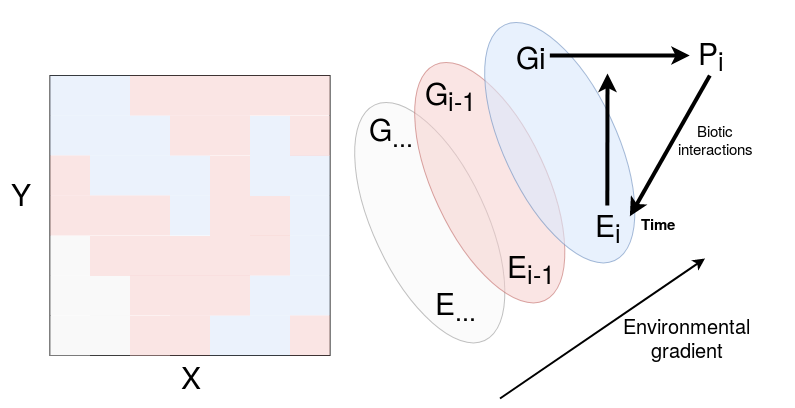
\includegraphics[width=\linewidth]{figures/phdscheme} 

}

\caption{Microgeographic adaptations among sympatric species within a species complex. Different genetic species $G$ grow in sympatry in specific habitats $E$ along an environmental gradient. The interaction of local environment $E_i$ and genotype $G_i$ result in phenotype $P_i$ . Phenotype $P_i$ feeds back to its local environment through biotic interactions. Temporal variation of the environment influences the phenotype of the established genotype.}\label{fig:phdscheme}
\end{figure}

To explore genotype-environment interactions, I needed first to characterise abiotic and biotic factors structuring ecological niches within and among species complexes (\(E_i\) in Fig. \ref{fig:phdscheme}).
I addressed the following question:

\textbf{\emph{\protect\hyperlink{Ch1}{Chapter 1}. How are species distributed within and among species complexes along biotic and abiotic gradients in Paracou?}}

I hypothesised species complexes to be widely spread across biotic and abiotic environments; whereas biotic and abiotic environments favour niche differentiation among species within species complexes.

To continue in the ecological theater, I needed to explore the role of abiotic and biotic environment on functional traits within and among closely-related species (\(E_i\) to \(P_i\) in Fig. \ref{fig:phdscheme}).
I addressed the following question:

\textbf{\emph{\protect\hyperlink{Ch2}{Chapter 2}. How does the abiotic environment influence individual leaf trait values among and within closely-related species within species complexes?}}

I hypothesised the abiotic environment to shape trait variation both among and within species in interaction with tree diameter and access to light within species complexes.

Once ecological niches defined and their relations with phenotypes explored, I could dive into individual and species adaptive genomics (\(E_i\times G_i\) to \(P_i\) in Fig. \ref{fig:phdscheme}).
I addressed individual and species adaptation to topography with the following question:

\textbf{\emph{\protect\hyperlink{Ch3}{Chapter 3}. Are tree species and individuals adapted to the fine-scale abiotic gradient?}}

I hypothesised species to be delimited along topography with fixed neutral and adaptive variants among and within species of species complexes.

Similarly, I addressed individual and species adaptation to forest gap dynamics with the following question:

\textbf{\emph{\protect\hyperlink{Ch4}{Chapter 4}. Are tree species and individuals adapted to a trade-off between growth and light access in response to forest gap dynamics?}}

I hypothesised individual genotypes to be adapted to a trade-off between growth and light access in response to forest gap dynamics.

Finally, once I explored the biotic and abiotic niches of individuals and species within species complexes, the resulting phenotypes and the underlying genomic adaptations, I was able to study the role of genotype-environment interactions in the coexistence of individuals and species within species complexes.
I addressed the following question:

\textbf{\emph{\protect\hyperlink{Discussion}{Discussion}. How do tree species' and individual's adaptations to microgeographic topography and forest gap dynamics drive coexistence within and among species of the \emph{Symphonia} species complex ?}}

I hypothesised genotypic adaptations within species of \emph{Symphonia} to decrease the risk of a stochastic local extinction due to wide successional niches which respond to fine spatio-temporal dynamics of forest gaps; and adaptations among species to stabilize local coexistence with differentiated species' topographic niches within the \emph{Symphonia} species complex.

\hypertarget{references}{%
\section*{References}\label{references}}
\addcontentsline{toc}{section}{References}

\hypertarget{refs}{}
\begin{CSLReferences}{1}{0}
\leavevmode\vadjust pre{\hypertarget{ref-hertzmann2000}{}}%
Hertzmann, A. and Zorin, D. 2000. Illustrating smooth surfaces (K Akeley, Ed.). - Proceedings of SIGGRAPH 2000 5: 517--526.

\end{CSLReferences}

% \addcontentsline{toc}{section}{References}
\bibliography{bib/thesis.bib}
% \listoftables
% \listoffigures

% Last pages

\end{document}
